\documentclass[11pt]{article}
\usepackage[margin=1in]{geometry}
\usepackage[utf8]{inputenc}
\usepackage[T1]{fontenc}
\usepackage{lmodern}
\usepackage{amsmath,amssymb,amsthm}
\usepackage{graphicx}
\usepackage{booktabs}
\usepackage{xcolor}
\usepackage{tikz}
\usetikzlibrary{positioning,arrows.meta,fit,calc,shapes.geometric}
\usepackage[hidelinks]{hyperref}
\usepackage{url}
\usepackage{caption}
\usepackage{subcaption}
\usepackage{enumitem}
\usepackage{longtable}
\usepackage{array}
\usepackage{listings}
\renewcommand{\topfraction}{0.9}
\renewcommand{\bottomfraction}{0.8}
\renewcommand{\textfraction}{0.07}
\renewcommand{\floatpagefraction}{0.75}
\setcounter{topnumber}{3}
\setcounter{totalnumber}{5}
\newsavebox{\fitbox}
\newcommand{\fittable}[1]{\sbox{\fitbox}{\input{#1}}%
  \ifdim\wd\fitbox>\linewidth\resizebox{\linewidth}{!}{\usebox{\fitbox}}\else\usebox{\fitbox}\fi}
\captionsetup{font=small,labelfont=bf}
\setlist{itemsep=1pt,topsep=3pt}
\setlist[description]{style=nextline,leftmargin=1.5em}
\emergencystretch=3em
\lstset{basicstyle=\ttfamily\footnotesize,columns=fullflexible,keepspaces=true,frame=none,
        xleftmargin=1em,showstringspaces=false}

\newcommand{\memprint}{MemPrint}
\newcommand{\term}[1]{\emph{#1}}
\newcommand{\code}[1]{\texttt{#1}}
\newcommand{\secref}[1]{Section~\ref{#1}}
\newcommand{\figref}[1]{Figure~\ref{#1}}
\newcommand{\tabref}[1]{Table~\ref{#1}}
\newcommand{\E}{\mathbb{E}}
\newcommand{\Var}{\mathrm{Var}}
\newcommand{\zhat}{\hat z}
\newtheorem{proposition}{Proposition}
\newcommand{\numfpExtra}{0.09}
\newcommand{\numfpInter}{0.27}
\newcommand{\numalphaExtra}{1.19}
\newcommand{\numalphaInter}{5.50}
\newcommand{\numownExtra}{18.04}
\newcommand{\numownInter}{10.85}
\newcommand{\numoracleExtra}{8.89}
\newcommand{\numoracleInter}{6.05}
\newcommand{\numrhoStaticExtra}{0.83}
\newcommand{\numrhoStaticInter}{0.85}
\newcommand{\numrhoAstExtra}{0.27}
\newcommand{\nummMedianErr}{0.85}
\newcommand{\numsdMedianErr}{13.82}
\newcommand{\numinterpMaxSeconds}{36.59}
\newcommand{\numrefShareMedian}{87.32}
\newcommand{\numautoFpMax}{2.24}
\newcommand{\numbigAutoAlphaMin}{0.77}
\newcommand{\numbigAutoAlphaMax}{4.65}
\newcommand{\numbigHandAlphaMin}{0.62}
\newcommand{\numbigHandAlphaMax}{4.08}
\newcommand{\numbigAutoFpMax}{0.44}
\newcommand{\nummaxScaleAuto}{18.00}


\title{From Source Code to Sampling Correction:\\Predicting Memory-Footprint Models for Unseen Programs}
\author{Nafis Mustakin\\University of California, Riverside}
\date{October 2026}

\begin{document}
\maketitle

\begin{abstract}
\memprint{} estimates how many bytes a program touches from a sparse sample of its memory references: a Pin
tool keeps one reference in $k$, and a regression model, trained on small inputs of the same program that were
traced completely, predicts the factor $\alpha$ by which the sampled footprint must be scaled up. The model
belongs to one program, so a program that has never been traced has no model. This report asks how a model can be
obtained for such an unseen program, and how the memory behaviour of two programs can be compared, when all that is
known about the new program is its source code. We show that, under Bernoulli sampling, $\alpha$ at every
sampling interval is a closed-form function of the program's \term{access-count spectrum}: how many bytes
receive how many references. We obtain that spectrum without running the program on its data, with a vectorised
abstract interpreter that executes the program's abstract syntax tree from \code{main()} and charges every memory
reference to its address, and we add a small, shared spectrum for the runtime (loader, C library, allocator),
fitted by non-negative least squares on other programs. On the 27 PolyBench kernels, with each kernel held out in
turn, this predicts the footprint within a median of \numfpExtra\% and \numfpInter\% (largest and middle input
held out) and $\alpha$ within a median of \numalphaExtra\% and \numalphaInter\%, against
\numownExtra\% and \numownInter\% for the kernel's own model trained on its traces and
\numoracleExtra\% and \numoracleInter\% for the best borrowed model chosen after the fact. A memory-behaviour
descriptor $z$ derived from the spectrum ranks which known model transfers best (median Spearman $\rho$ of
\numrhoStaticExtra{}--\numrhoStaticInter), as well as the descriptor measured from traces and far better than
counts of syntax-tree nodes ($\rho=\numrhoAstExtra$). For irregular programs, whose memory behaviour depends on
their input, we extend the approach in three steps on the GAP graph benchmarks: a hand-written skeleton that replays
the program on an input drawn from the distribution of its generator (blind tests on Kronecker graphs, new kernels
and OpenMP threads pass with 0.6--11\% error), an interpreter that runs irregular C code, and finally a C++
interpreter that runs GAP's own source for all six kernels on both graph families at scales 10--18, predicting the
footprint within 3\% and $\alpha$ within about a point of the hand-written skeleton for pr, bfs and tc. A blind test
on two programs never used in development, with predictions committed before they were traced, passes clearly on
HPCCG (footprint within 2.1\%, $\alpha$ within 0.5--4.4\%, against 11--12\% for its own model) and partly on LULESH
(footprint within 4.2\%, $\alpha$ within 5\% at small and middle meshes but 28--43\% at the largest). We describe
every component in enough detail to re-implement it, and we report the limitations, the post-hoc corrections and the
parts of the evaluation that are not blind.
\end{abstract}

\tableofcontents
\listoffigures
\listoftables
\newpage

%=====================================================================
\section{Introduction}
\label{sec:intro}

The memory footprint of a program, the number of distinct bytes it touches during a run, decides how many jobs fit
on a node, how large a cache or memory tier must be, and whether a program fits in device memory at all. The direct
way to measure it is to record every memory reference with a dynamic binary instrumentation tool such as
Pin~\cite{Luk2005Pin}; this costs two to three orders of magnitude in run time. \memprint{}~\cite{memprint}
reduces that cost by recording only a random subset of the references: each reference is kept with probability $1/k$.
The bytes touched by the kept references, the \term{sampled footprint} $m$, underestimates the true footprint, because
bytes that are referenced only a few times are often missed. \memprint{} learns the correction: for each program it
fits a regression model that predicts the ratio $\alpha = \text{truth}/m$ from $m$, $k$ and the spread of $m$ across
independent subsamples, using small inputs of the same program that were traced completely.

That model is specific to one program. Its training needs complete traces of that program at several input sizes;
a program that was never traced has no model. A natural idea is to reuse the model of a similar program, but this
raises two questions that this report answers:

\begin{enumerate}
\item \textbf{Similarity.} Given models for programs $A$, $B$ and $D$ and a new program $C$ whose memory behaviour
``falls between'' $B$ and $D$, how can memory-behaviour similarity be quantified so that it predicts which model
transfers?
\item \textbf{From code.} If nothing is known about $C$ except its source code, which static features of the code
determine where $C$ falls, and how does the code translate into the memory-behaviour descriptor $z(C)$?
\end{enumerate}

Our answer to both is the same object, the \term{access-count spectrum} of the program (\secref{sec:theory}). Under
Bernoulli sampling, the spectrum determines the mean and variance of the sampled footprint at every interval $k$ in
closed form. It therefore determines $\alpha$ directly (no model needs to be borrowed at all), it defines a
descriptor $z$ in which distances between programs predict transfer error, and it can be computed from source code by
abstract interpretation~\cite{cousot1977}.

\paragraph{Contributions.}
\begin{itemize}
\item A derivation showing that $\alpha$, the bins' spread and their unique-address counts follow from the spectrum
(\secref{sec:theory}), and a descriptor $z$ of memory behaviour with two parts, \term{reuse} and \term{spread}
(\secref{sec:descriptor}).
\item A vectorised abstract interpreter for C that computes the spectrum from source (\secref{sec:interp}), a
shared runtime baseline fitted by non-negative least squares (\secref{sec:baseline}), and an access-idiom gate that
recognises code outside the interpreter's reach (\secref{sec:gate}).
\item A leave-one-workload-out evaluation on 27 PolyBench kernels comparing eleven ways to predict an unseen kernel
(\secref{sec:pb}).
\item An extension to irregular, input-dependent code on the GAP benchmark suite~\cite{beamer2015gap}: a skeleton
replay on inputs sampled from the generator's distribution, with blind tests (\secref{sec:skeleton}), an
interpreter for irregular C (\secref{sec:interp-c}) and a C++ interpreter that runs GAP's unmodified source
(\secref{sec:cpp}).
\end{itemize}

\figref{fig:pipeline} shows the whole pipeline. \secref{sec:background} defines the terms used throughout;
\tabref{tab:glossary} collects them.

\begin{figure}[!htbp]
\centering
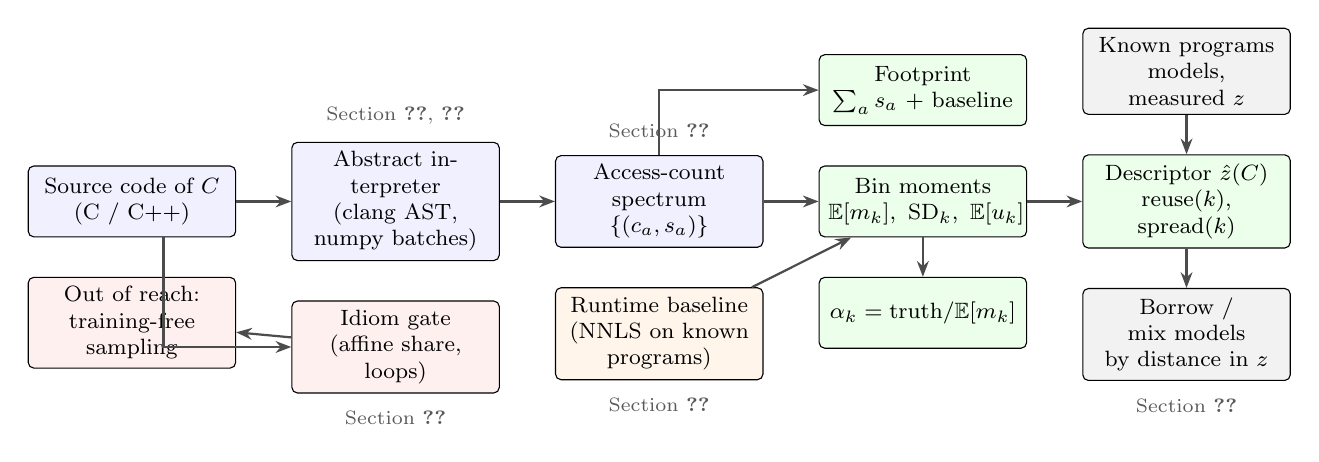
\begin{tikzpicture}[
  node distance=5mm and 7mm,
  box/.style={draw, rounded corners=2pt, align=center, font=\footnotesize, minimum height=9mm, text width=24mm,
              fill=#1},
  box/.default=white,
  arrow/.style={-{Stealth[length=2mm]}, thick, draw=black!70},
  lab/.style={font=\scriptsize, text=black!65, align=center}]
\node[box=blue!6] (src) {Source code of $C$\\(C / C++)};
\node[box=blue!6, right=of src] (interp) {Abstract interpreter\\(clang AST, numpy batches)};
\node[box=blue!6, right=of interp] (spec) {Access-count spectrum\\$\{(c_a, s_a)\}$};
\node[box=orange!8, below=of spec] (base) {Runtime baseline\\(NNLS on known programs)};
\node[box=green!8, right=of spec] (mom) {Bin moments\\$\E[m_k],\ \mathrm{SD}_k,\ \E[u_k]$};
\node[box=green!8, above=of mom] (fp) {Footprint\\$\sum_a s_a$ + baseline};
\node[box=green!8, below=of mom] (alpha) {$\alpha_k = \text{truth}/\E[m_k]$};
\node[box=green!8, right=of mom] (z) {Descriptor $\hat z(C)$\\reuse$(k)$, spread$(k)$};
\node[box=gray!10, above=of z] (known) {Known programs\\models, measured $z$};
\node[box=gray!10, below=of z] (borrow) {Borrow / mix models\\by distance in $z$};
\node[box=red!6, below=of interp] (gate) {Idiom gate\\(affine share, loops)};
\node[box=red!6, below=of src] (fallback) {Out of reach:\\training-free sampling};
\draw[arrow] (src) -- (interp);
\draw[arrow] (interp) -- (spec);
\draw[arrow] (spec) -- (mom);
\draw[arrow] (base) -- (mom);
\draw[arrow] (spec) |- (fp);
\draw[arrow] (mom) -- (alpha);
\draw[arrow] (mom) -- (z);
\draw[arrow] (known) -- (z);
\draw[arrow] (z) -- (borrow);
\draw[arrow] (src.south) ++(4mm,0) |- ($(gate.west)+(0,0)$);
\draw[arrow] (gate) -- (fallback);
\node[lab, above=1mm of interp] {\secref{sec:interp}, \ref{sec:cpp}};
\node[lab, above=1mm of spec] {\secref{sec:theory}};
\node[lab, below=1mm of base] {\secref{sec:baseline}};
\node[lab, below=1mm of gate] {\secref{sec:gate}};
\node[lab, below=1mm of borrow] {\secref{sec:descriptor}};
\end{tikzpicture}
\caption[The prediction pipeline]{The prediction pipeline for an unseen program $C$. Blue: computed from $C$'s
source alone. Orange: fitted on other programs. Green: quantities that follow in closed form. Gray: what borrowing a
known model needs. Red: the check that sends code the analysis cannot handle to a training-free method.}
\label{fig:pipeline}
\end{figure}

%=====================================================================
\section{Background and terminology}
\label{sec:background}

\subsection{References, addresses and the footprint}

A \term{memory reference} (or \term{access}) is one load or store executed by the program; it covers a byte range
$[\text{addr}, \text{addr}+\text{size})$. An \term{address} in this report is a 4-byte \term{unit}: the
interpreter and the skeletons count references per aligned 4-byte unit, and a reference counts once for every unit it
covers, whatever its width. The \term{footprint} of a run is the number of distinct bytes covered by at least one
reference (\term{bytes touched}). This is \memprint{}'s \code{-footprint bytes} mode. The original definition,
\code{-footprint starts}, adds up the largest access size seen at each start address and counts overlapping accesses
more than once; we use bytes touched throughout, and all traces in this report were recorded with it.

\subsection{The splitter and its bins}

\memprint{}'s Pin tool in \term{splitter} mode records every reference of a run once and produces, from that single
run, both the exact footprint and many subsamples. For each \term{sampling interval}
$k \in \mathcal{K} = \{100, 250, 500, 750, 1000, 2500, 5000, 7500, 10^4, 2.5\cdot 10^4, 5\cdot 10^4,
7.5\cdot 10^4, 10^5\}$ it keeps $B=20$ \term{bins}. Each bin keeps every reference independently with probability
$1/k$ (a Bernoulli subsample, drawn with an independent random stream per bin). For a bin the tool reports:
\begin{itemize}
\item \code{MemUsageObs}, the \term{bin footprint} $m$: the bytes touched by the bin's references;
\item \code{UniqueAddresses} $u$: the number of distinct addresses among them;
\item \code{CountObs}: the number of references the bin kept.
\end{itemize}
The interval $k=1$ is the complete trace: its \code{MemUsageObs} is the true footprint, \term{truth}. The tables
of all bins of all inputs of a program are the program's \term{traces} (\code{allData} files).

\subsection{The correction factor $\alpha$ and the per-program model}
\label{sec:model}

For one bin at interval $k$, $\alpha = \text{truth}/m$. \memprint{} predicts it with a log-linear model with
interactions:
\begin{equation}
\log\alpha = b_0 + b_1 \ell_\sigma + b_2 \ell_k + b_3 \ell_m + b_4 \ell_m\ell_\sigma + b_5 \ell_k\ell_\sigma
+ b_6 \ell_m \ell_k + b_7 \ell_m\ell_\sigma\ell_k ,
\label{eq:model}
\end{equation}
with $\ell_\sigma = \log \mathrm{SD}_k$ (the standard deviation of $m$ across the $B$ bins of that interval),
$\ell_k = \log k$ and $\ell_m = \log m$. Rows with $k \in \{1,10\}$ and intervals with an empty bin are dropped.
Training uses the other inputs of the same program. We call this the program's \term{own model}.

\subsection{Inputs, splits and error}

Each program has several \term{configs} (input sizes), ordered by true footprint. Two \term{splits} are evaluated:
\term{EXTRA} holds out the largest config (extrapolation) and \term{INTER} the middle one (interpolation). Accuracy is
the \term{MAPE}, the mean absolute percentage error of predicted $\alpha$ against measured $\alpha$ over all bins
of all 13 intervals at the held-out config; for the footprint it is the absolute percentage error of the predicted
truth.

\subsection{Workloads}
\begin{itemize}
\item \textbf{PolyBench/C 4.2.1}~\cite{polybench}: 27 kernels (all but deriche, durbin and jacobi-1d, as in the
original \memprint{} study), each at seven sizes: MINI, MINI2, MINI3, SMALL, SMALL2, SMALL3, MEDIUM. Built
\code{-O0}. Affine loop nests over arrays.
\item \textbf{GAP}~\cite{beamer2015gap} (commit \code{b5e3e19}), built with its default \code{-O3}: pr
(PageRank, 20 iterations, \code{-t 0}), prc (PageRank to convergence, \code{-t 1e-4}), bfs (direction-optimising
BFS~\cite{beamer2012dobfs}), cc (Afforest~\cite{sutton2018afforest}), sssp
($\Delta$-stepping~\cite{meyer2003delta}), tc (triangle counting) and bc (Brandes~\cite{brandes2001}), on
synthetic graphs generated inside the program: \term{uniform} (\code{-u $s$}) or \term{Kronecker}
(\code{-g $s$}, R-MAT~\cite{chakrabarti2004rmat,leskovec2010kronecker}) with $2^s$ vertices and average degree 16,
at \term{scales} $s=10,\dots,18$. pr and bfs were also run with 4 OpenMP threads.
\item \textbf{miniVite}~\cite{minivite} (graph community detection, MPI), as a transfer check.
\item Two small C programs written for this work, \code{csr\_pr.c} and \code{csr\_bfs.c}.
\end{itemize}

\begin{table}[!htbp]
\centering\small
\caption{Glossary of the terms used in this report.}
\label{tab:glossary}
\begin{tabular}{>{\raggedright\arraybackslash}p{0.24\linewidth}>{\raggedright\arraybackslash}p{0.7\linewidth}}
\toprule
Term & Meaning \\
\midrule
reference, access & one executed load or store, covering a byte range \\
address, unit & an aligned 4-byte unit; references are counted per unit they cover \\
footprint, truth & bytes touched by the whole run (\code{-footprint bytes}) \\
sampling interval $k$ & each reference is kept with probability $1/k$ \\
bin & one independent 1-in-$k$ subsample of a run; 20 per interval \\
bin footprint $m$ & bytes touched by a bin's references (\code{MemUsageObs}) \\
$\mathrm{SD}_k$, spread & standard deviation of $m$ across the bins of interval $k$ \\
$\alpha$ & truth$/m$, the factor that scales a sampled footprint up \\
own model & \eqref{eq:model} fitted on the program's other inputs \\
config, scale & an input size; for GAP the scale $s$ means $2^s$ vertices \\
EXTRA, INTER & largest / middle config held out \\
MAPE & mean absolute percentage error over all bins at the held-out config \\
access-count spectrum & the multiset $\{(c_a, s_a)\}$: address $a$ of $s_a$ bytes receives $c_a$ references \\
inclusion probability & $p(c,k)=1-(1-1/k)^c$, the chance a bin holds an address with $c$ references \\
runtime baseline & spectrum of what the loader, C library and allocator touch, outside the program text \\
descriptor $z$, $\hat z$ & reuse$(k)$ and spread$(k)$ over the 13 intervals; measured ($z$) or predicted ($\hat z$) \\
coverage & share of charged references that the interpreter placed exactly \\
uncertain, unresolved & reference under data-dependent control / at a data-dependent address \\
batch, batch point & a set of loop iterations executed together as numpy arrays / one of them \\
skeleton & a hand-written numpy replay of a program's memory behaviour \\
gate & the idiom check that decides whether the static prediction is trusted \\
LOWO & leave one workload out: every program is held out in turn \\
blind & the model was committed before the workload it predicts was traced \\
\bottomrule
\end{tabular}
\end{table}

%=====================================================================
\clearpage
\section{The access-count spectrum decides $\alpha$}
\label{sec:theory}

\subsection{Moments of a bin}

Let the run reference address $a$ (of $s_a$ bytes) $c_a$ times. A bin keeps each of the $c_a$ references
independently with probability $1/k$, so address $a$ is in the bin unless all its references were dropped:
\begin{equation}
p_a = p(c_a, k) = 1 - \left(1 - \tfrac1k\right)^{c_a}.
\label{eq:p}
\end{equation}
The bin footprint is $m = \sum_a s_a X_a$ with independent indicators $X_a \sim \mathrm{Bernoulli}(p_a)$, hence
\begin{equation}
\E[m] = \sum_a s_a\, p_a, \qquad
\Var[m] = \sum_a s_a^2\, p_a (1-p_a), \qquad
\E[u] = \sum_a p_a, \qquad
\text{truth} = \sum_a s_a .
\label{eq:moments}
\end{equation}
We predict $\alpha_k$ by $\text{truth}/\E[m_k]$ and the spread by $\sqrt{\Var[m_k]}$. The ratio of expectations
differs from the expectation of the ratio by a second-order term in $\Var[m]/\E[m]^2$, which is below $10^{-3}$ for
all bins in our data except the sparsest bins of the smallest inputs. The spectrum is all that is needed: two
programs with the same spectrum have the same $\alpha$ curve, whatever their code.

\begin{proposition}
For any spectrum, $1 \le \alpha_k \le k$, with $\alpha_k = k$ exactly when every address is referenced once
and $\alpha_k \to 1$ when every address is referenced many more than $k$ times.
\end{proposition}
\begin{proof}
$p(1,k) = 1/k$ and $p(c,k)$ increases in $c$ towards 1, so $1/k \le p_a \le 1$; hence
$\text{truth}/k \le \E[m] \le \text{truth}$.
\end{proof}

\figref{fig:inclusion} shows both effects. An address enters a bin with probability $1 - 1/e \approx 0.63$ when it is
referenced $c=k$ times; the transition from ``almost never'' to ``almost always'' spans about two decades of $c$
around $k$. The $\alpha$ curve of a program is therefore a readout of how its bytes are spread over reference
counts: the bytes referenced far fewer than $k$ times dominate $\alpha_k$.

\begin{figure}[!htbp]
\centering
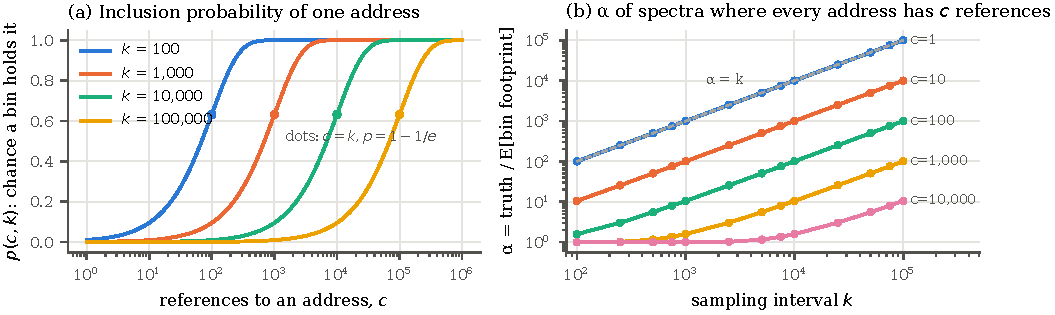
\includegraphics[width=\linewidth]{figures/inclusion.pdf}
\caption[Inclusion probability and the $\alpha$ of idealised spectra]{(a) The probability that a 1-in-$k$ bin holds
an address referenced $c$ times, \eqref{eq:p}. (b) $\alpha_k$ for spectra in which every 4-byte address is referenced
exactly $c$ times: $\alpha_k \approx k/c$ while $c \ll k$, and $\alpha_k \to 1$ once $c \gg k$.}
\label{fig:inclusion}
\end{figure}

\subsection{Assumptions}
\begin{itemize}
\item \textbf{Independence.} The splitter draws each reference's inclusion independently (per bin, with its own
pseudo-random stream), so the $X_a$ are independent. A deterministic 1-in-$k$ sampler (every $k$-th reference) would
instead interact with the program's periodicity; \memprint{}'s spread term would then carry aliasing effects that the
spectrum alone does not determine.
\item \textbf{Time does not matter.} $\alpha$ of a whole-run footprint depends only on how often each address is
referenced, not when. (Footprint over time, with memory freed, needs the timing as well; see the companion
report~\cite{timeline2026}.)
\item \textbf{Address reuse.} When the allocator reuses an address range for a new block, the references to both
blocks count for the same addresses. The interpreter and the skeletons therefore place heap blocks as glibc does
(\secref{sec:heap}).
\end{itemize}

\subsection{A descriptor of memory behaviour}
\label{sec:descriptor}

For comparing programs we summarise the bin statistics at one config by a descriptor with two parts, each a curve
over the 13 intervals:
\begin{equation}
\text{reuse}(k) = \frac{\log \alpha_k}{\log k}, \qquad
\text{spread}(k) = \log\frac{\mathrm{SD}_k}{\E[m_k]} .
\label{eq:z}
\end{equation}
reuse$(k)$ is 1 when no address is referenced twice ($\alpha_k = k$) and falls towards 0 under heavy reuse; it is
dimensionless and comparable across programs of very different size. spread$(k)$ is the bins' coefficient of
variation on a log scale. The descriptor $z(W) \in \mathbb{R}^{26}$ is \term{measured} from a program's traces;
$\zhat(W)$ is \term{predicted} by evaluating \eqref{eq:moments} on the static spectrum plus the runtime baseline.
The distance between two programs is the Euclidean distance after standardising every component with the mean and
standard deviation of the known programs (missing components are set to the mean). We ask in \secref{sec:pb} whether
this distance predicts how well one program's model transfers to the other.

%=====================================================================
\clearpage
\section{Computing the spectrum from source code}
\label{sec:interp}

\subsection{Overview}

The interpreter (\code{analysis/memprint/static/interp.py}, about 1{,}500 lines of Python) parses the program
with libclang~\cite{libclang} through its C API (ctypes), and executes the abstract syntax tree (AST) from
\code{main()} without the program's input data. It is an abstract interpreter in the sense of
\cite{cousot1977}: values are either exact integers or the abstract value $\top$ (\code{UNK}, unknown), and every
memory reference the program would make is \term{charged} to its address. The result is the per-address reference
count, i.e.\ the spectrum, plus counts of what could not be placed.

\subsection{Values and memory}
\begin{itemize}
\item \textbf{Integers} (sizes, loop indices, flags) are tracked exactly as Python integers or numpy \code{int64}
arrays. Conversions to C types wrap to the type's width and signedness (\code{wrap\_int}).
\item \textbf{Floating-point values} are unknown in the C interpreter; the C++ interpreter tracks floating-point
\emph{scalars} (\secref{sec:cpp-values}).
\item \textbf{Memory objects} (\code{Obj}): the stack, globals, \code{.rodata} and every heap block. Each keeps
per-access-size reference counts per byte offset, so that counts can later be folded into 4-byte units, and, for
irregular code, the integer values stored in it (one \code{int64} per 4-byte unit, plus a byte array for objects
smaller than 4 bytes), with a sentinel for ``unknown''.
\item \textbf{Pointers} are pairs (object, byte offset); the offset may be an array (one per batch point).
\end{itemize}

\subsection{Batches: running a loop nest all at once}

A counted loop (a \code{for} loop whose bound and step are known integers) does not run iteration by iteration. The
interpreter computes its trip count for every enclosing batch point and runs the body once for all iterations
together: the loop variable becomes a numpy array, and every expression in the body is evaluated element-wise. A
statement in a nest of depth $d$ is thus executed once, with one batch point per iteration of the nest. Batches are
processed in chunks of at most $2^{21}$ points (\code{CHUNK}). Each batch point carries a weight $w$, so a statement
charges $\sum w$ references; weights below 1 express uncertainty (below). This makes MEDIUM PolyBench inputs
(up to $3.6 \times 10^9$ references) take at most \numinterpMaxSeconds\,s (\figref{fig:pb-cost}a).

\paragraph{Loops that cannot be batched.}
\begin{itemize}
\item \textbf{General loops} (\code{while}, \code{do}, \code{for} with an unknown bound) run one iteration at a
time for all batch points still in the loop: each iteration evaluates the condition per point and drops the points
for which it is false (\code{\_loop\_general}). A cap of $2^{24}$ iterations guards against runaway loops.
\item \textbf{Loops carried through memory}: a loop whose body reads and then writes an integer array (a prefix
sum, a BFS claiming vertices) gives different values if its iterations are batched. If it is not nested in another
such loop and has at most $2\times 10^6$ iterations (\code{SEQUENTIAL\_LIMIT}), it runs one iteration at a time;
otherwise it stays batched, and the values it computes may differ from a sequential run.
\item \textbf{Repeated indices}: \code{a[i]++} and \code{a[i] += x} in a batched loop keep their sequential meaning
when several batch points hit the same element (degree counting, \code{nbr[pos[u]++] = v}): the updates are
applied in iteration order with a stable sort and a cumulative sum per element (\code{\_rmw\_add}); \code{|=},
\code{\&=} and \code{\^{}=} with repeated offsets reduce with \code{ufunc.at}.
\end{itemize}

\subsection{What is charged (\code{-O0})}

PolyBench is traced at \code{-O0}, where every variable lives in memory. The C interpreter therefore charges:
reads and writes of locals and parameters (stack slots, at the offsets a frame layout pass assigns; frames at the same
call depth share addresses, \code{FRAME\_BYTES}${}=8192$), array elements, floating-point constants (each distinct
constant gets a \code{.rodata} slot), and each call's return address and saved frame pointer. Local arrays larger
than 1{,}024 bytes get their own object. The interpreter charges a median of \numrefShareMedian\% of the references
Pin observes (\figref{fig:pb-cost}b); the remainder is additional \code{-O0} stack traffic of gcc (spills,
temporaries) on a few addresses that are referenced so often that every bin samples them, which leaves $\alpha$
unchanged.

\subsection{Uncertainty and coverage}

The interpreter does not guess. A branch whose condition is unknown executes both arms, each with half the weight,
and marks their references \term{uncertain}; a loop with an unknown trip count runs its body once
(\code{GUESS\_TRIPS}${}=1$), uncertain. A reference whose address depends on unknown data is \term{unresolved}: it is
counted but not placed. \term{Coverage} is the share of references that are neither. All PolyBench kernels reach a
coverage of 1.0 since integer values in memory are tracked; before that, floyd-warshall and nussinov, whose branches
compare values computed in memory, had 0.77.

\subsection{Irregular C: memory values, random numbers, the heap}
\label{sec:interp-c}
\label{sec:heap}

To run programs whose control depends on data they compute (graph codes), the interpreter also:
\begin{itemize}
\item remembers integer values stored in memory, so loops bounded by loaded values (\code{row[v+1]}) and
subscripts that load an index (\code{A[B[i]]}) resolve;
\item draws \code{rand()}, \code{random()} and \code{lrand48()} from their distributions with a seeded generator,
and charges the C library's own references per call: a microbenchmark under Pin measured about 27 references per
call, 24 to about 120 bytes of generator state and 3 to its 31-word table;
\item places heap blocks as glibc 2.28 does (\code{skeleton.Process}, described in \secref{sec:skeleton}), so that addresses reused by later blocks are counted once.
\end{itemize}

\subsection{Implementation constants}

\begin{table}[!htbp]
\centering\small
\caption{Constants of the interpreters and skeletons.}
\label{tab:constants}
\begin{tabular}{l>{\raggedleft\arraybackslash}p{0.22\linewidth}>{\raggedright\arraybackslash}p{0.45\linewidth}}
\toprule
Name & Value & Role \\
\midrule
\code{UNIT} & 4 B & counting granularity \\
\code{CHUNK} & $2^{21}$ & batch points per chunk \\
\code{MAX\_ITERATIONS} & $2^{24}$ & iterations of a general loop before giving up \\
\code{SEQUENTIAL\_LIMIT} & $2\times10^6$ & iterations a memory-carried loop may run one at a time \\
\code{GUESS\_TRIPS} & 1 & trips charged for a loop with unknown trip count \\
\code{FRAME\_BYTES} & 8192 & stack frame size (\code{-O0}) \\
\code{STACK\_ARRAY\_LIMIT} & 1024 B & larger local arrays get their own object \\
\code{REGISTER\_BYTES} & 64 B & C++ objects up to this size live in registers (\code{-O3}) \\
\code{MMAP\_THRESHOLD} & 128 KiB (dynamic, $\le$ 32 MiB) & glibc's mapping threshold \\
\code{TOP\_PAD} & 128 KiB & heap growth pad \\
\code{MINSIZE} & 32 B & smallest chunk \\
\code{HEAP\_TOP\_AT\_START} & 59{,}328 B & free bytes in the top chunk at a GAP program's first large allocation \\
\bottomrule
\end{tabular}
\end{table}

%=====================================================================
\clearpage
\section{The runtime baseline}
\label{sec:baseline}

A traced run also touches memory that the program text does not describe: the dynamic loader, C library
initialisation, \code{stdio} buffers, allocator metadata. We model it as one spectrum shared by all programs of the
same runtime: $b_j$ bytes in $n_j$ addresses referenced $c_j = 2^j$ times, $j=0,\dots,26$. Its contribution to the
moments is \eqref{eq:moments} summed over the 27 classes (addresses of a class have $b_j/n_j$ bytes). The coefficients
are fitted by non-negative least squares~\cite{lawson1974} to the residuals of the known programs: for every known
program, config and interval, the observed mean bin footprint minus the static prediction,
\[
\min_{b \ge 0} \sum_{(W,\text{cfg},k)} \left( \frac{\bar m_{\text{obs}} - \E[m]_{\text{static}} - \sum_j b_j\,
p(c_j, k)}{\bar m_{\text{obs}}} \right)^2 ,
\]
plus one row per config at $k=1$ whose target is the true footprint. Residuals are relative so that small and large
inputs weigh alike. The addresses $n_j$ are fitted in the same way on unique-address counts. In the leave-one-out
evaluation the baseline is refitted every time without the held-out program.

Fitted on all 27 PolyBench kernels, the baseline has 105~KB, almost all referenced once, plus about 3~KB
referenced 32--512 times; for GAP's C++ runtime (libstdc++, \code{-O3}) it has 463~KB (\figref{fig:baseline},
\tabref{tab:baseline}). The baseline matters most for small inputs: it is half the footprint of GAP at scale 10.

\begin{figure}[!htbp]
\centering
\begin{minipage}[b]{0.49\linewidth}
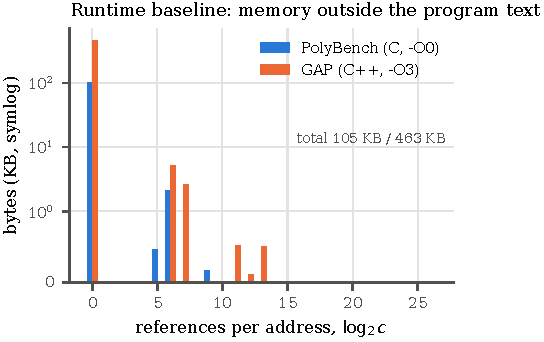
\includegraphics[width=\linewidth]{figures/baseline.pdf}
\caption[Runtime baselines]{Runtime baselines fitted by NNLS: bytes per reference-count class.}
\label{fig:baseline}
\end{minipage}\hfill
\begin{minipage}[b]{0.49\linewidth}
\centering\scriptsize
\fittable{tables/baseline.tex}
\captionof{table}[Runtime baseline coefficients]{Non-zero baseline classes.}
\label{tab:baseline}
\end{minipage}
\end{figure}

%=====================================================================
\clearpage
\section{Using the spectrum for an unseen program}
\label{sec:methods}

Given the static spectrum $S_C$ of the unseen program $C$ at its test config and the baseline $b$:

\begin{description}
\item[static footprint] $\text{truth} \approx \sum_a s_a + \sum_j b_j$. No sampling at all.
\item[static $\alpha$] $\alpha_k \approx \text{truth}/\E[m_k]$ from \eqref{eq:moments}, evaluated at the interval
of each bin. (The bin's own observed $m$ is not needed.)
\item[pooled regression] one model \eqref{eq:model} over all known programs, with $\log$ static $\alpha$ as an
eighth feature.
\item[nearest model by $\zhat$] the own model of the known program $W$ closest to $\zhat(C)$.
\item[RBF mixture by $\zhat$] the known models' $\log\alpha$ predictions averaged with weights
$w_W \propto \exp(-d(\zhat_C, z_W)^2 / 2h^2)$, with bandwidth $h$ the median nearest-neighbour distance among the
known programs.
\end{description}

Four references complete the comparison: the same two borrowing schemes with $C$'s \emph{measured} $z$ (an upper
bound for $\zhat$), the nearest model by distance in clang AST node counts (the baseline static feature: the
$\log(1+\text{count})$ of every node kind), a uniform mixture of all known models (no similarity), $C$'s own model
(which needs $C$'s traces) and the \term{oracle}, the known model with the lowest error on $C$, chosen after scoring.

\subsection{The access-idiom gate}
\label{sec:gate}

The static prediction is trustworthy where the interpreter places the references, i.e.\ for code close to the affine
kernels it was validated on. A separate pass over the AST (\code{static/idioms.py}) classifies every memory
reference by how its address is formed: \term{affine} (subscripts built from integer variables, constants, $+$, $-$
and multiplication by a constant), \term{indirect} (a subscript that loads memory or calls a function:
\code{A[B[i]]}, CSR neighbours, hash lookups), \term{pointer} (dereference or \code{->}) or \term{other}; and every
loop as \term{counted}, \term{data-bounded} (bound is a load that depends on an enclosing loop variable,
\code{e < row[v+1]}) or \term{while}. References are weighted by $10^{\text{loop depth}}$ as a static stand-in for
their dynamic count. The gate sends a program to training-free sampling if the interpreter's coverage is below 0.5,
the affine share below 0.95, or more than 5\% of loops are data-bounded or while loops.

%=====================================================================
\clearpage
\section{Evaluation on PolyBench}
\label{sec:pb}

\subsection{Protocol}

Every kernel $C$ is held out in turn (leave one workload out, LOWO; \code{analysis/memprint/lowo.py}). Only $C$'s
source is used to predict; $C$'s traces are used only for scoring and for the reference methods that are marked as
using them. The 26 other kernels provide the baseline, their own models (fitted on all their configs) and their
measured $z$ (at the config of the same name as $C$'s test config). The test config is MEDIUM (EXTRA) or SMALL2
(INTER). Static spectra for all $27\times7$ kernel--config pairs are computed once
(\code{python -m memprint static spectra}).

\subsection{Accuracy}

\begin{table}[!htbp]
\centering\small
\caption[Leave-one-out accuracy on PolyBench]{Leave-one-workload-out MAPE (\%) of $\alpha$ on the held-out kernel,
27 kernels. The first row is the footprint error. ``Uses'' says what each method needs beyond the known programs.}
\label{tab:lowo}
\fittable{tables/lowo.tex}
\end{table}

\tabref{tab:lowo} and \figref{fig:lowo} give the results; \tabref{tab:lowo-kernel} in the appendix lists every
kernel.

\begin{itemize}
\item \textbf{Predicting beats borrowing.} Static $\alpha$ is within a median of \numalphaExtra\% (EXTRA) and
\numalphaInter\% (INTER). The kernel's own model, trained on its own traces at smaller inputs, has \numownExtra\% and
\numownInter\%, and even the oracle, the best borrowed model picked after seeing the errors, has \numoracleExtra\% and
\numoracleInter\%. \figref{fig:static-vs-own} shows that the source beats the own model on almost every kernel under
EXTRA, where the own model has to extrapolate.
\item \textbf{The static footprint is nearly exact} (median \numfpExtra\% / \numfpInter\%; \figref{fig:pb-fp}). The
worst cases are correlation, gramschmidt and cholesky at their INTER size (1.7--2.6\%).
\item \textbf{The pooled regression} with static $\alpha$ as a feature is worse than static $\alpha$ alone: the
regression's other features add the known programs' idiosyncrasies.
\item \textbf{Similarity helps when borrowing}: choosing a model by $\zhat$ cuts the error of the uniform mixture by a
factor of 4--8.
\end{itemize}

\begin{figure}[!htbp]
\centering
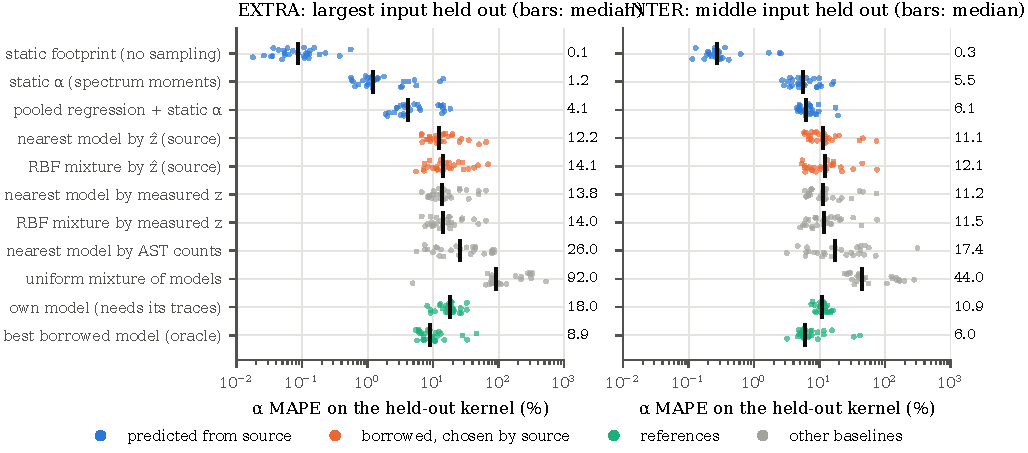
\includegraphics[width=\linewidth]{figures/lowo_methods.pdf}
\caption[Leave-one-out errors by method]{Leave-one-out MAPE of every method on each held-out kernel (dots; bars and
numbers: medians). Blue: predicted from the source. Orange: a known model chosen by $\zhat$. Green: references that
need the held-out kernel's traces. Gray: other baselines.}
\label{fig:lowo}
\end{figure}

\begin{figure}[!htbp]
\centering
\begin{minipage}[t]{0.49\linewidth}
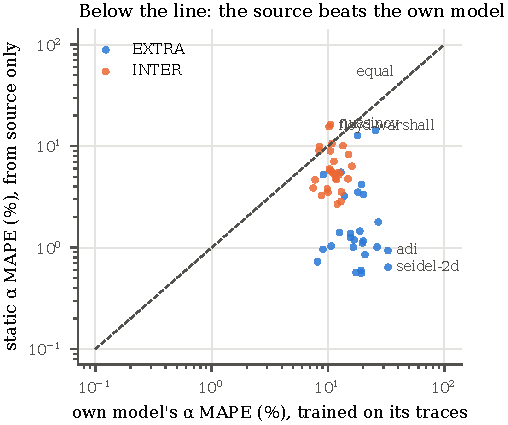
\includegraphics[width=\linewidth]{figures/pb_static_vs_own.pdf}
\caption[Static $\alpha$ against the own model]{Static $\alpha$ error (from the source only) against the own model's
error (trained on the kernel's traces), per kernel and split.}
\label{fig:static-vs-own}
\end{minipage}\hfill
\begin{minipage}[t]{0.49\linewidth}
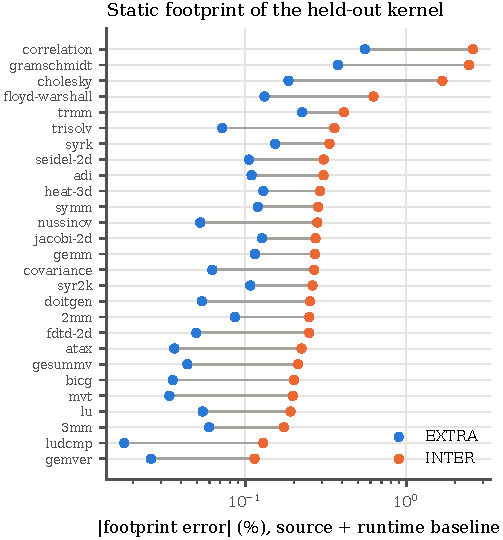
\includegraphics[width=\linewidth]{figures/pb_footprint.pdf}
\caption[Static footprint error per kernel]{Footprint predicted from the source plus the runtime baseline, per
held-out kernel.}
\label{fig:pb-fp}
\end{minipage}
\end{figure}

\subsection{The moments match Pin}

\figref{fig:alpha-curves} overlays the predicted $\alpha_k$ curve on every bin Pin recorded, for nine kernels at
MEDIUM, and \figref{fig:moments} compares all three predicted moments with the measured ones over every kernel,
config and interval. The mean bin footprint is predicted within a median of \nummMedianErr\%. The spread is
predicted within a median of \numsdMedianErr\%, systematically a little low (\figref{fig:sd-error}): with $B=20$
bins the sample standard deviation itself has a relative standard error of about 16\%, so most of the scatter is the
measurement's. The unique-address count agrees except for floyd-warshall and nussinov, where the interpreter's unit
granularity and Pin's start-address count differ by a factor of about 4; $\alpha$ does not use it.

\figref{fig:alpha-heatmap} shows the static $\alpha$ error at every size: it is largest at the smallest inputs,
where the runtime baseline is a large part of the footprint, and for the two kernels with data-dependent
\code{min}/\code{max} ternaries, floyd-warshall and nussinov (12.8--16.3\%). Their outer loops now run sequentially,
but their inner loops stay batched, so the values that decide the branches may differ from a sequential run.

\begin{figure}[!htbp]
\centering
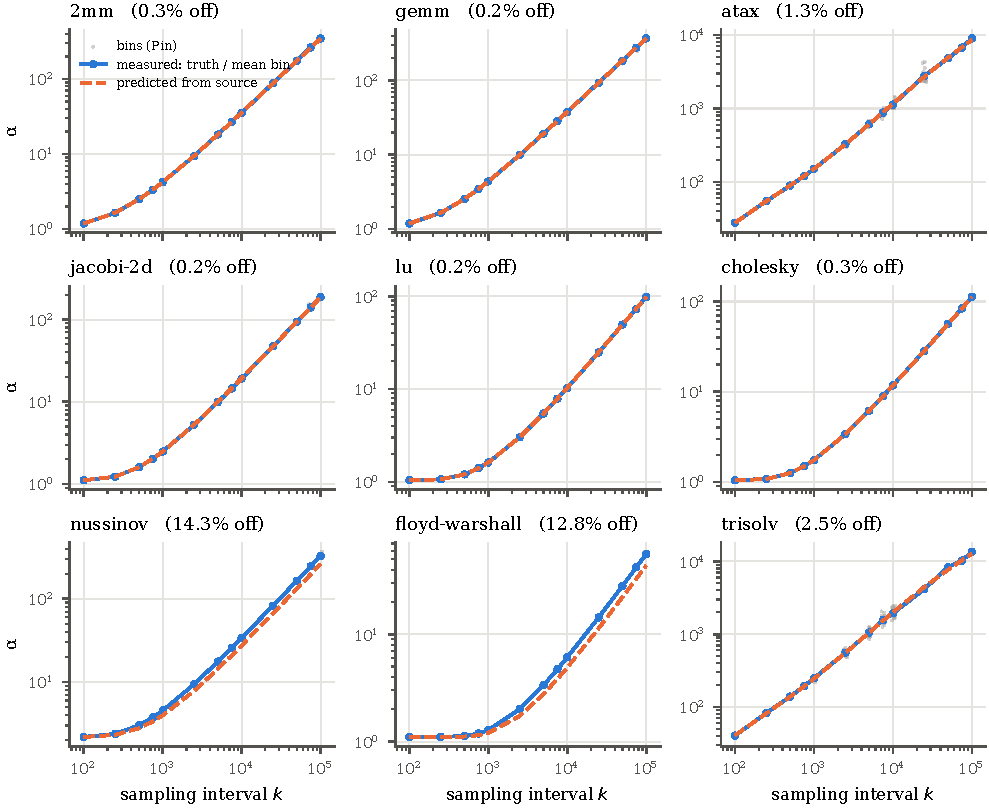
\includegraphics[width=\linewidth]{figures/pb_alpha_curves.pdf}
\caption[Predicted and measured $\alpha$ curves on PolyBench]{$\alpha$ against the sampling interval at MEDIUM:
every Pin bin (gray), the measured truth over the mean bin footprint (blue) and the prediction from the source
(orange, dashed). The title gives the MAPE over the 13 intervals.}
\label{fig:alpha-curves}
\vspace{1em}
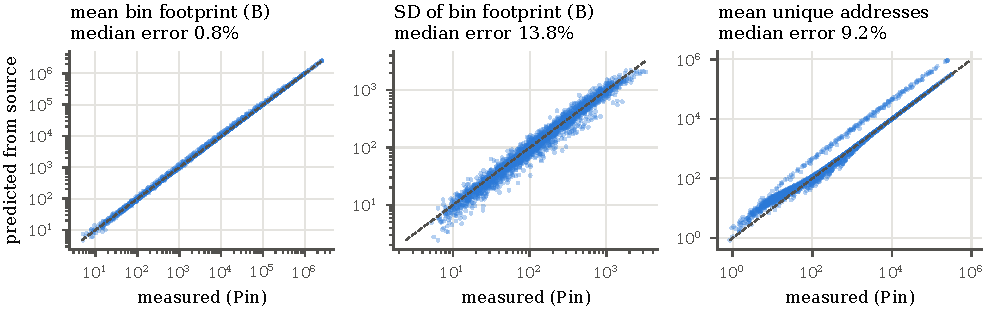
\includegraphics[width=\linewidth]{figures/pb_moments_scatter.pdf}
\caption[Predicted against measured bin moments]{The three moments of \eqref{eq:moments}, predicted from source
against measured, for every kernel, config and interval (2{,}457 points).}
\label{fig:moments}
\end{figure}

\begin{figure}[!htbp]
\centering
\begin{minipage}[t]{0.47\linewidth}
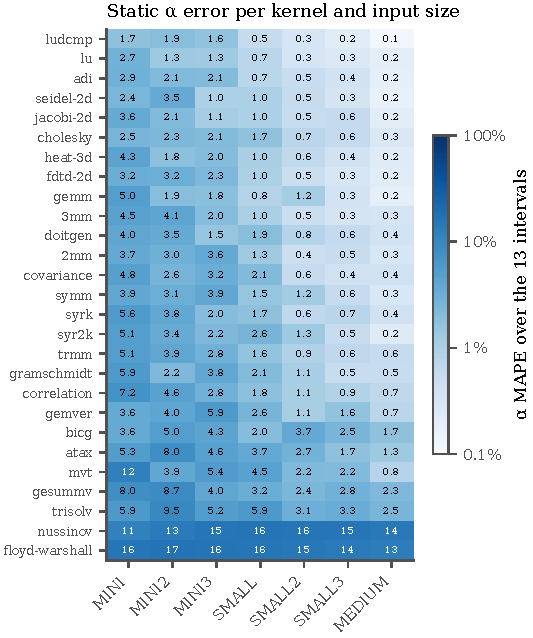
\includegraphics[width=\linewidth]{figures/pb_alpha_heatmap.pdf}
\caption[Static $\alpha$ error per kernel and size]{Static $\alpha$ MAPE per kernel and input size (baseline fitted
without the kernel).}
\label{fig:alpha-heatmap}
\end{minipage}\hfill
\begin{minipage}[t]{0.5\linewidth}
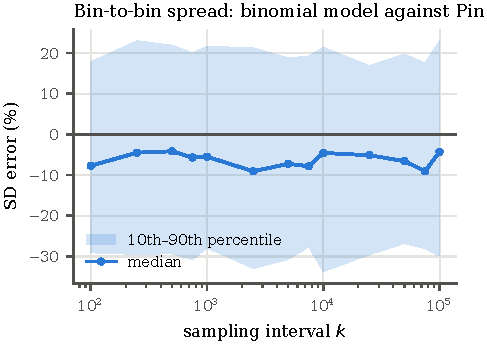
\includegraphics[width=\linewidth]{figures/pb_sd_error.pdf}
\caption[Error of the predicted spread]{Signed error of the predicted standard deviation of the bin footprint, by
interval.}
\label{fig:sd-error}
\vspace{0.6em}
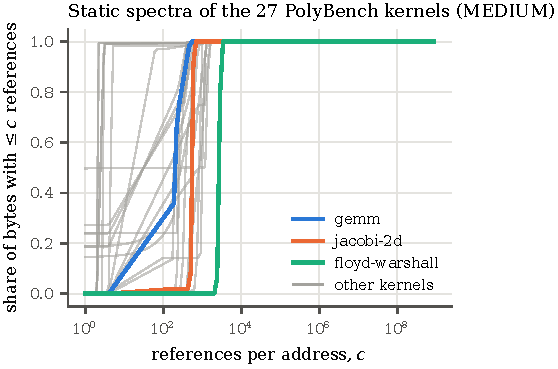
\includegraphics[width=\linewidth]{figures/pb_spectra.pdf}
\caption[Static spectra of PolyBench]{Cumulative static spectra at MEDIUM: the share of bytes referenced at most $c$
times.}
\label{fig:pb-spectra}
\end{minipage}
\end{figure}

\subsection{Similarity: does $\zhat$ rank transferable models?}

For each held-out kernel we compute the Spearman rank correlation~\cite{spearman1904} between the distance from $C$
to each known kernel and the error of that kernel's model on $C$. A high $\rho$ means that nearer programs have
models that transfer better.

\begin{table}[!htbp]
\centering\small
\caption{Spearman $\rho$ between descriptor distance and transfer error, over the 27 held-out kernels.}
\label{tab:similarity}
\fittable{tables/similarity.tex}
\end{table}

$\zhat$ ranks the transferable models as well as the measured $z$ does, and much better than AST node counts
(\tabref{tab:similarity}, \figref{fig:similarity}a). This answers the first question of the introduction: the
spectrum-derived descriptor is a usable similarity, and it can be computed from code. $\zhat$ is also close to $z$ in
absolute terms: the median RMSE of reuse$(k)$ is 0.0014, at most 0.032 (\figref{fig:similarity}b,
\figref{fig:reuse}).

\begin{figure}[!htbp]
\centering
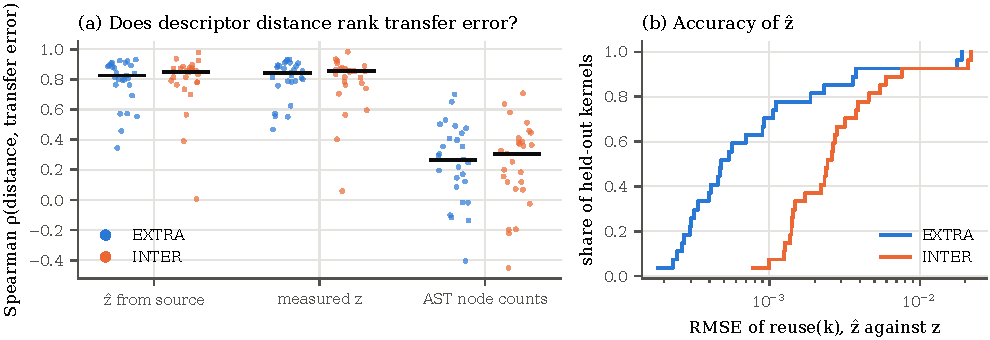
\includegraphics[width=\linewidth]{figures/similarity.pdf}
\caption[Validity of the descriptor]{(a) Spearman $\rho$ between descriptor distance and transfer error, one dot
per held-out kernel (bars: medians). (b) Cumulative distribution of the RMSE between $\zhat$ and $z$ on reuse$(k)$.}
\label{fig:similarity}
\end{figure}

\begin{figure}[!htbp]
\centering
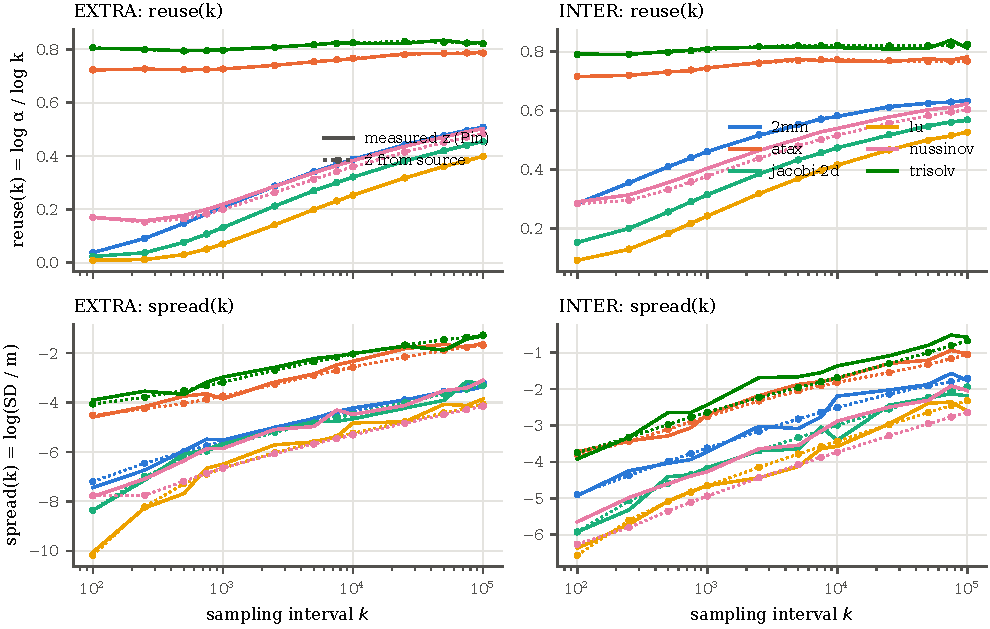
\includegraphics[width=\linewidth]{figures/reuse_curves.pdf}
\caption[Predicted and measured descriptor curves]{The two parts of the descriptor, measured (solid) and predicted
from source (dotted), for six kernels.}
\label{fig:reuse}
\end{figure}

\subsection{Cost}

\figref{fig:pb-cost}a shows the interpreter's run time against the number of references it charges: below 0.2\,s up to
$10^7$ references, then roughly linear, at most \numinterpMaxSeconds\,s. A full Pin trace of the same MEDIUM inputs
takes minutes.

\begin{figure}[!htbp]
\centering
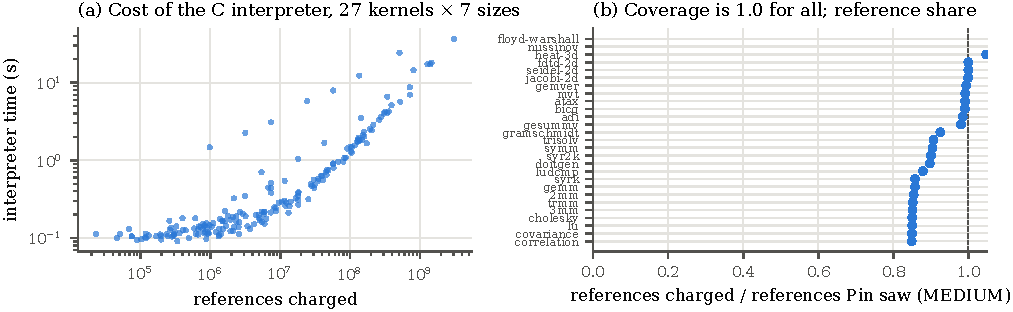
\includegraphics[width=\linewidth]{figures/pb_interp_cost.pdf}
\caption[Cost and reference share of the C interpreter]{(a) Interpreter time per kernel and config. (b) References the
interpreter charges as a share of those Pin records, at MEDIUM. Coverage is 1.0 for every kernel.}
\label{fig:pb-cost}
\end{figure}

\subsection{The gate on irregular programs}

\begin{table}[!htbp]
\centering\small
\caption{Access idioms of PolyBench and of irregular programs.}
\label{tab:idioms}
\fittable{tables/idioms.tex}
\end{table}

All PolyBench kernels pass the gate; miniVite, GAP and darknet fail it (\tabref{tab:idioms}, \figref{fig:idioms}).
On miniVite the call is right (\figref{fig:minivite}): its own model has 11.4\% error at its largest input, the
PolyBench model nearest by measured $z$ (3mm) 64.5\%, the best PolyBench model chosen after the fact 46.3\% and the
median one 80.0\%. Its measured $z$ is 4.3 from the nearest PolyBench kernel, where PolyBench kernels' own
nearest-neighbour distances are at most 1.84, so the descriptor flags it as out of distribution as well.

\begin{figure}[!htbp]
\centering
\begin{minipage}[t]{0.49\linewidth}
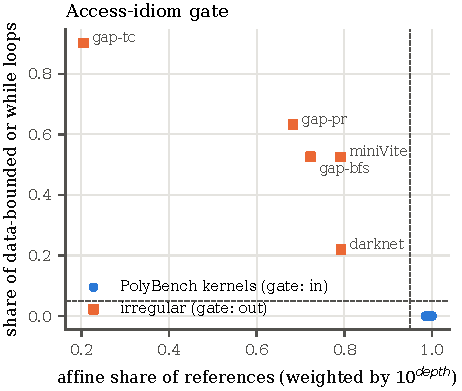
\includegraphics[width=\linewidth]{figures/idioms.pdf}
\caption[The access-idiom gate]{Affine share against the share of data-bounded or while loops. Dashed: the gate's
thresholds.}
\label{fig:idioms}
\end{minipage}\hfill
\begin{minipage}[t]{0.49\linewidth}
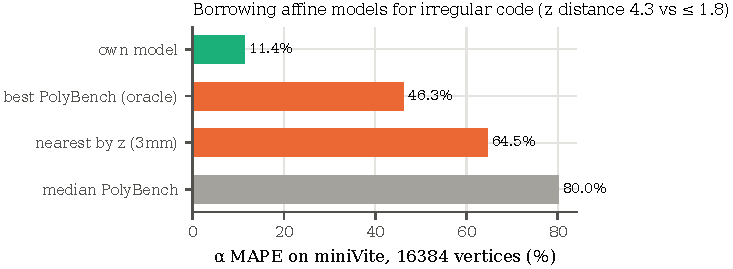
\includegraphics[width=\linewidth]{figures/minivite.pdf}
\caption[Borrowing PolyBench models for miniVite]{Errors on miniVite of its own model and of borrowed PolyBench
models.}
\label{fig:minivite}
\end{minipage}
\end{figure}

%=====================================================================
\clearpage
\section{Irregular code I: a skeleton and the input's distribution}
\label{sec:skeleton}

In an irregular program the access counts depend on the input: a vertex is read once per neighbour. Yet benchmark
inputs are often \emph{generated} by the program itself from a known distribution, as in GAP. The spectrum then
depends only on the generator's distribution, which the source states. We first test this idea with hand-written
\term{skeletons} (\code{static/skeleton.py}, \code{static/gap.py}, \code{static/gap\_kernels.py}, about 900 lines),
and then replace them with interpreters (\secref{sec:cpp}).

\subsection{The input distribution}

GAP generates its graphs inside the program: \code{MakeUniformEL} draws both endpoints of every edge uniformly with a
Mersenne Twister~\cite{matsumoto1998mt} (\code{std::mt19937}, reseeded every $2^{18}$ edges); \code{MakeRMatEL}
draws, per edge and per depth, one 32-bit number that selects a quadrant with probabilities $A=0.57$,
$B=C=0.19$, then permutes the vertex IDs with \code{std::shuffle}. The skeleton draws its graph from the same
distribution with numpy (not GAP's actual edges). \figref{fig:degrees} shows the resulting degree distributions:
Poisson-like for uniform graphs, heavy-tailed for Kronecker graphs.

\subsection{The skeleton}

A skeleton is a numpy replay of the program's memory behaviour on the sampled input. A \code{Process} object provides
\code{new(bytes)}, \code{delete(block)} and \code{touch(block, index, elem\_size, refs)}, which adds reference counts
per 4-byte unit. For GAP it replays:
\begin{itemize}
\item \textbf{The builder}: edge-list generation, \code{FindMaxNodeID} (an extra read of the edge list because
\code{num\_nodes\_} starts at $-1$), degree counting with atomic increments, a prefix sum, CSR construction,
\code{SquishCSR} (sort, unique and remove of every neighbour list), and symmetrisation.
\item \textbf{The kernels}: pr's 20 iterations; bfs's top-down and bottom-up steps and direction switches on the
sampled graph; cc's Afforest (Link, Compress, 1{,}024-sample guess of the largest component); sssp's
$\Delta$-stepping with per-bin vectors on the weighted builder; tc's \code{WorthRelabelling},
\code{RelabelByDegree} and \code{OrderedCount}; bc's Brandes from one source; prc's convergence loop, with its
iteration count obtained by running the \code{float32} update on the sampled graph. Sequential parts run in
numba~\cite{lam2015numba}.
\item \textbf{Library costs}, measured outside GAP: \code{std::sort} references per element along a curve measured
under Pin for lists of 2--16{,}384 integers (\tabref{tab:sortrefs}); \code{lock xadd} as a read and a write; the
Mersenne Twister's 624 state words of 8 bytes, each referenced $2$ times per seeding and $4\cdot\text{draws}/624$ times
per batch of draws.
\end{itemize}

\begin{table}[!htbp]
\centering\small
\caption[Measured references per element of \code{std::sort}]{References per element of \code{std::sort} on $d$
random 4-byte integers, measured under Pin (g++ 8.5, \code{-O3}); interpolated in $\log_2 d$.}
\label{tab:sortrefs}
\begin{tabular}{l*{10}{r}}
\toprule
$d$ & 2 & 4 & 8 & 16 & 32 & 64 & 256 & 1024 & 4096 & 16384 \\
refs/element & 3.25 & 5.55 & 8.22 & 12.61 & 13.52 & 15.41 & 19.08 & 23.09 & 26.60 & 30.77 \\
\bottomrule
\end{tabular}
\end{table}

\subsection{The glibc heap model}

Because the footprint counts an address once however many blocks occupy it, where blocks are placed matters. The
model follows glibc 2.28~\cite{glibcmanual}: a request of $n$ bytes needs a chunk of $\max(32, \lceil
(n+8)/16\rceil\cdot16)$ bytes; it is served best-fit from free heap chunks, else from the top chunk; only when the top
chunk is too small does the size decide between a mapping (at or above the mmap threshold) and growing the heap by the
request plus a 128~KiB pad, rounded to pages. Freed chunks coalesce, and into the top chunk when adjacent; a free that
leaves more than the trim threshold in the top chunk returns memory to the OS down to the pad. Freeing a mapping
raises the mmap threshold to its size (up to 32~MiB) and the trim threshold to twice that. Under Pin, holes left by
\code{munmap} are not reused (the tool's own mappings take them), which the model reproduces. The heap's starting
state, 59{,}328 free bytes in the top chunk at GAP's first large allocation (libstdc++'s 72{,}704-byte emergency pool
and the command line are already there), was measured once with \code{mallinfo()} from an \code{LD\_PRELOAD} shim.
At scale 14, a 131~KB array lands on the heap or in a mapping by a margin of about 2~KB; this model brought the
footprint error there from 1.8\% to under 0.4\%.

\subsection{Calibration and blind tests}

The uniform-graph pr and bfs results are \emph{not} blind: two corrections were found by comparing against their
traces (generated graphs are always symmetrised, \code{symmetrize\_ = true}; the generator state uses 8-byte words).
Three further corrections were measured outside GAP (the sort curve, the cost of \code{lock xadd} and glibc's
placement). Everything after that was tested \textbf{blind}: the model was committed before the workloads it predicts
were traced, and not changed after scoring. The blind tests were: Kronecker graphs for pr and bfs (only the generator
was added), the five further kernels cc, sssp, tc, bc and prc on both graph families, and pr and bfs with 4 OpenMP
threads (per-thread generators and arenas, per-thread queue buffers). One disclosure: for prc, the native iteration
counts were printed before the freeze commit; the replay was not changed.

\subsection{Results}

\begin{table}[!htbp]
\centering\scriptsize
\caption[Skeleton results on GAP]{GAP skeleton: footprint error and $\alpha$ MAPE (\%) at the held-out scale (EXTRA:
18, INTER: 14), against the workload's own model and borrowed PolyBench models (nearest by $\zhat$, uniform mean,
oracle). The baseline is fitted on other GAP workloads.}
\label{tab:gap}
\fittable{tables/gap_pilot.tex}
\end{table}

\tabref{tab:gap} and \figref{fig:gap-methods} summarise the 36 held-out tests. The skeleton beats each workload's own
model in 28 of them; borrowed PolyBench models are 16--98\% off. The footprint is predicted within 0.0--2.9\% at
every scale (\figref{fig:gap-fp}). The blind Kronecker test passes with $\alpha$ within 1.2--2.2\%, more accurate
than on uniform graphs, presumably because the skewed degrees move more of the footprint into hub vertices and long
neighbour lists, which the replay gets right (an untested explanation). sssp (7.3--11.3\%) and tc (9.0--11.2\%) are
worse than their own models; their coarsest parts are sssp's per-bin vectors and tc's merge loops, whose cost depends
on how \code{-O3} keeps the iterator in a register. Threads did not make prediction harder (0.8--4.5\%): every array
access is the same as in the serial run. \figref{fig:gap-scales} shows the error at every scale; it falls with scale
for pr, bfs and cc, as the runtime baseline becomes a smaller part of the footprint.

\begin{figure}[!htbp]
\centering
\begin{minipage}[t]{0.49\linewidth}
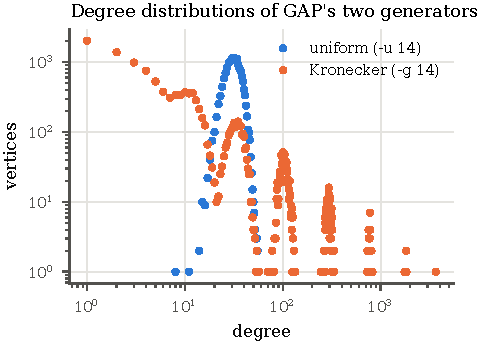
\includegraphics[width=\linewidth]{figures/gap_degrees.pdf}
\caption[Degree distributions of GAP's generators]{Degree distributions of the graphs drawn from GAP's two
generators at scale 14.}
\label{fig:degrees}
\end{minipage}\hfill
\begin{minipage}[t]{0.49\linewidth}
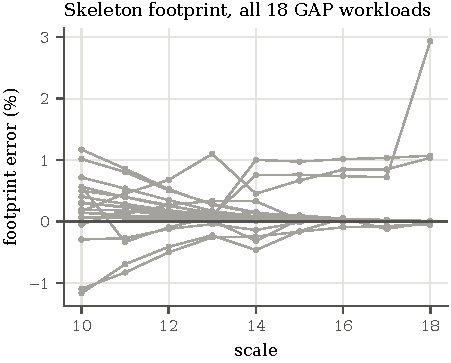
\includegraphics[width=\linewidth]{figures/gap_footprint.pdf}
\caption[Skeleton footprint error]{Skeleton footprint error at every scale, all GAP workloads.}
\label{fig:gap-fp}
\end{minipage}
\end{figure}

\begin{figure}[!htbp]
\centering
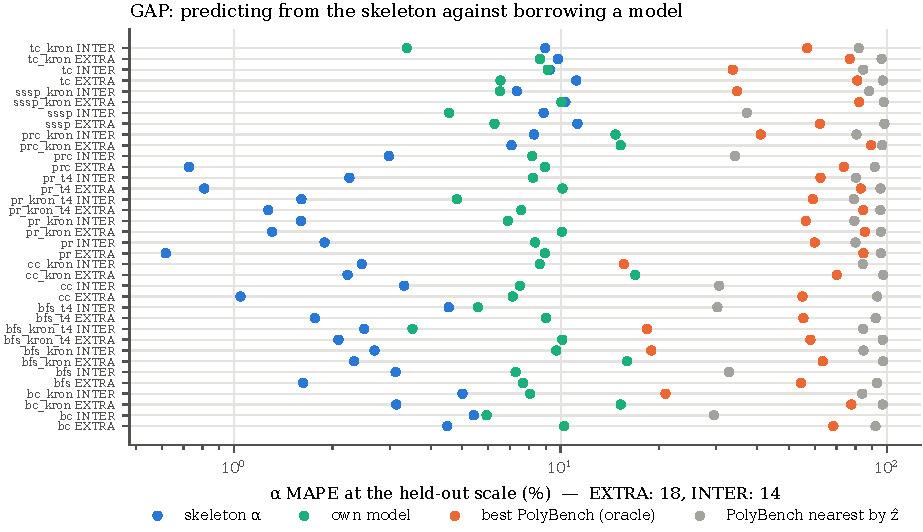
\includegraphics[width=\linewidth]{figures/gap_methods.pdf}
\caption[GAP: skeleton against borrowed models]{GAP: $\alpha$ error of the skeleton, the workload's own model and the
borrowed PolyBench models, per workload and split.}
\label{fig:gap-methods}
\end{figure}

\begin{figure}[!htbp]
\centering
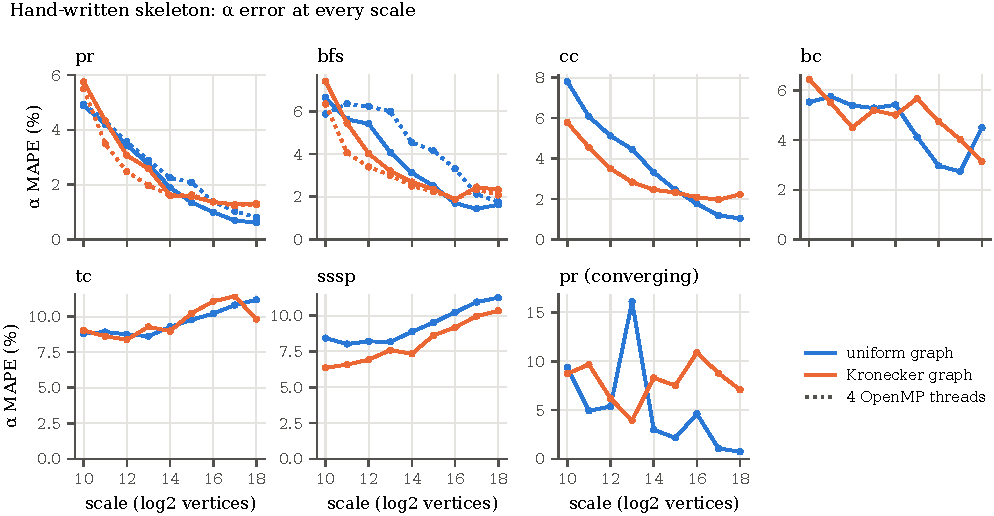
\includegraphics[width=\linewidth]{figures/gap_skeleton_scales.pdf}
\caption[Skeleton error per scale]{Skeleton $\alpha$ MAPE at every scale, for the seven kernels, both graph families
and (pr, bfs) 4 threads.}
\label{fig:gap-scales}
\end{figure}

\subsection{Irregular C programs run by the interpreter}

The interpreter of \secref{sec:interp-c} was tested on two C programs written for the purpose, \code{csr\_pr.c} and
\code{csr\_bfs.c}: both build a random CSR graph from \code{rand()}, then run PageRank or a queue-driven BFS. They
were built \code{-O0} and traced at scales 8--16 (pr) and 8--14 (bfs); the baseline was fitted on PolyBench. The blind
run missed the C library's internal references per \code{rand()} call; adding the measured cost brought $\alpha$ to
1.3--6.0\% (\tabref{tab:csr}, \figref{fig:csr}). That correction is post hoc.

\begin{figure}[!htbp]
\centering
\begin{minipage}[b]{0.5\linewidth}
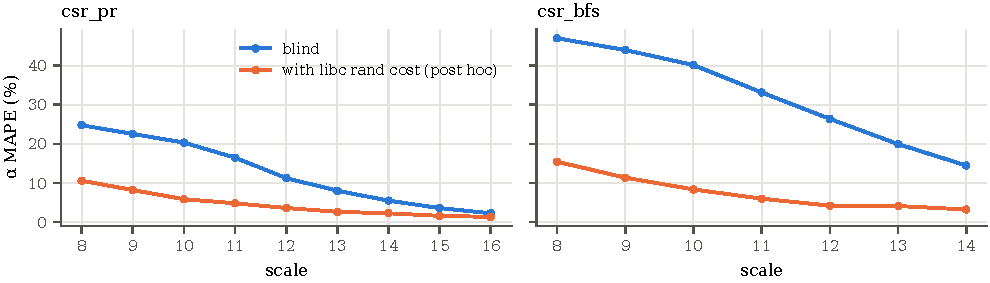
\includegraphics[width=\linewidth]{figures/csr_programs.pdf}
\caption[Interpreter on irregular C programs]{$\alpha$ MAPE per scale of the interpreter on two irregular C programs,
blind and with the libc \code{rand()} cost.}
\label{fig:csr}
\end{minipage}\hfill
\begin{minipage}[b]{0.47\linewidth}
\centering\scriptsize
\fittable{tables/csr.tex}
\captionof{table}[Interpreter on irregular C programs]{Footprint and $\alpha$ MAPE (\%) on the two C programs.}
\label{tab:csr}
\end{minipage}
\end{figure}

%=====================================================================
\clearpage
\section{Irregular code II: interpreting GAP's C++ source}
\label{sec:cpp}

The skeletons work but are written by hand. The C++ interpreter (\code{static/interp\_cpp.py}, about 2{,}000 lines,
and \code{static/containers.py}) removes that step: it runs GAP's unmodified source, from \code{main()}, through
the command-line parser, the generator and builder, the kernel and the destructors.

\subsection{Object model}
\begin{itemize}
\item \textbf{Objects and members.} Fields sit at the offsets libclang reports; \code{this} is a pointer; member
calls, operators and lambdas' \code{operator()} are dispatched on the referenced declaration. libclang's
\code{get\_arguments()} omits the object of an operator call; whether it is included is decided by comparing the
argument count with the callee's parameter count.
\item \textbf{Construction and destruction.} Constructors run member initialisers, default member initialisers and
delegation; an implicitly defined \code{operator=} (no parameter declarations in the AST) is executed as a
member-wise copy. Objects returned by value are constructed in storage the caller provides (sret); a returned local
is not destroyed. Destructors run at scope exit (libclang does not show those calls).
\item \textbf{References} hold the address they bind to; a call that returns a reference is an lvalue. A scalar bound
to a reference (an out-parameter such as \code{\&index}) is materialised in memory.
\item \textbf{Pointers in memory} are remembered as (object, offset) per 4-byte unit, so arrays of pointers such as
GAP's CSR index resolve.
\item \textbf{Templates.} libclang gives instantiated function bodies with concrete types; for class-template
patterns the interpreter resolves fields on the concrete type.
\item \textbf{Function values.} A function passed to a template parameter (tc passes \code{Hybrid} to
\code{BenchmarkKernel}) evaluates to a function value, and a call through a variable holding one invokes its
definition.
\end{itemize}

\subsection{Values}
\label{sec:cpp-values}
\begin{itemize}
\item \textbf{Floating-point values} (\code{Real}) are tracked through literals, casts, arithmetic, comparisons and
the C math functions (\code{pow}, \code{sqrt}, \code{cbrt}, \code{exp}, \code{log}, \code{fabs}, \code{floor},
\dots), in scalars and in memory: every memory object keeps a float per 4-byte unit beside its integers (NaN when
unknown; an integer store forgets it, and a unit whose integer value is 0 reads as 0.0). So a decision such as tc's
\code{sample\_average / 1.3 > sample\_median}, or a problem parameter stored in a struct, resolves. A floating-point
compound update of memory (\code{f[node[e]] += x}) is applied in iteration order with \code{np.add.at}, so repeated
indices accumulate as in a sequential loop. A constant floating-point expression converted to an integer is folded
by clang (\code{const uint32\_t A = 0.57*max}).
\item \textbf{Per-point values at one address.} A local array in the body of a batched loop has one address for all
iterations (which is right for counting), but each iteration writes its own values. When a batch stores an array of
values to a single address, the object keeps them per point, and a load from that address by a batch of the same
size returns each point's value.
\item \textbf{Partial values.} A variable assigned in the branches of an \code{if}/\code{else} that different batch
points take is known per point once every point has been assigned (\code{Partial}); before, it became unknown. (Added
after the blind test, \secref{sec:blind}.)
\end{itemize}

\subsection{Counting as \code{-O3} does}

GAP is traced at \code{-O3}, where most scalars never touch memory. The interpreter therefore:
\begin{itemize}
\item keeps scalar locals and objects of at most 64 bytes (an \code{Edge}, a \code{Neighborhood}, a
\code{pvector}'s three pointers) in a per-batch-point register file whose accesses are not charged; taking such an
object's address or binding it to a reference moves it to memory;
\item eliminates redundant loads per batch point: a point's load of a location it (or the point it derives from in
an enclosing batch) already accessed through the same base pointer, with no store to that object since, is free.
Every batch records, per (object, access size, base-pointer provenance), the offset each point loaded, and links to
the batch it was derived from: a subset of its points, the iterations of a vectorised loop, or one iteration of a
loop run one at a time. Loads before a loop are therefore hoisted out of it (loop-invariant code motion), an
iteration does not reuse what the previous one loaded, and the latest value a \code{while} condition loaded is kept
for after the loop (tc's \code{while (*it < w) it++;} followed by \code{w == *it}). Provenance is the object a
pointer was loaded from (and, for a small object, the field), the same in every batch. A store forgets every entry
of its object; a library call that may write memory forgets everything.
\end{itemize}

\subsection{The standard library}

The standard library is modelled, not interpreted (its declarations are recognised by
\code{is\_in\_system\_header}):
\begin{itemize}
\item \code{std::vector}: three pointers (start, finish, end of storage) as in libstdc++; buffers come from one arena
object so that a batched loop over many vectors works on one object; \code{push\_back} grows by doubling (copy,
release); \code{resize} value-initialises new elements, and nested vectors start as empty vectors.
\item \code{std::unordered\_map}: nodes (key, value) of 16 bytes in the arena; bucket arrays are not modelled.
\item \code{std::sort} (field-wise lexicographic order, \code{std::greater} descending; cost from
\tabref{tab:sortrefs}), \code{unique}, \code{remove}, \code{copy} (whole elements move), \code{fill},
\code{shuffle} (libstdc++ 8's two-positions-per-draw variant), \code{swap}, \code{max\_element}, \code{min},
\code{max}, \code{numeric\_limits}, \code{std::pair} and \code{make\_pair};
\item \code{std::mt19937} and \code{uniform\_int\_distribution}: values (a generator per call site, seeded as in the
source) and the state-word costs of \secref{sec:skeleton};
\item GAP's atomic helpers \code{fetch\_and\_add} and \code{compare\_and\_swap} (and the GCC builtins): applied in
iteration order across batch points, so the first point to reach a location wins, as in a sequential run.
\end{itemize}
Streams and strings are ignored; command-line accessors come from a table of stubs (scale, degree, graph family,
number of trials).

\subsection{Control flow}
\begin{itemize}
\item \code{break} and \code{continue} are per-loop flags; a loop whose body may break runs one iteration at a time for
the batch points still in it (\code{\_loop\_with\_break}, \code{\_range\_with\_break}). A \code{break} under a
condition on unknown (floating-point) data is ignored, so the loop runs to its bound; this is exact for pr with
\code{-t 0} and an upper bound for converging loops.
\item \code{range-for} runs through \code{begin()}/\code{end()} as a batch, sequentially if it carries values
through memory.
\item When only some batch points run a statement (after a partial \code{break}), the statement runs on that subset;
variables it declares are merged back to the full batch.
\item \textbf{Reductions and scans.} A loop whose carried scalar is only summed, or set to \code{min}/\code{max} of
itself, runs as one batch and combines the iterations per enclosing point. A loop whose carried integer or pointer
is only changed by increments that do not read it (\code{v += x}, \code{v++}, \code{*p++ = x}), anywhere in the
body including branches and nested loops, and that no condition reads, is a \term{scan}: a first pass that charges
and stores nothing (and restores every variable) gives each iteration's increment, and each iteration then starts
from $v_0$ plus the increments of the earlier iterations of its enclosing point. GAP's prefix sum and HPCCG's
row-by-row matrix generation run this way instead of one iteration at a time.
\item \textbf{Loop conditions.} In a conjunction (\code{k < max\_iter \&\& normr > tolerance}), a part that compares
floating-point values and is unknown is taken as true when the other parts are known, so the loop runs to its
integer bound, consistent with the rule for \code{break}.
\end{itemize}

Programs of several source files are compiled as one unity file (headers without an include guard get
\code{\#pragma once}); the command line is given as strings (\code{argv}; \code{atoi}, \code{strtol},
\code{std::stoi}, \code{strcmp} and \code{strlen} read them); class-type fields without an initialiser are
default-constructed (\code{std::vector} members start empty).

\subsection{Bugs found by comparing against the hand skeleton}

Comparing the interpreter's heap blocks, one by one, with the skeleton's exposed interpreter errors that a footprint
check alone would have hidden. \tabref{tab:bugs} lists those that changed results.

\begin{table}[!htbp]
\centering\small
\caption{Interpreter defects found on GAP and their fixes.}
\label{tab:bugs}
\begin{tabular}{>{\raggedright\arraybackslash}p{0.35\linewidth}>{\raggedright\arraybackslash}p{0.6\linewidth}}
\toprule
Symptom & Cause and fix \\
\midrule
sssp ran forever & \code{vector<vector<int>>::operator[]} returns the typedef \code{reference}; it was not recognised as a
reference, so each bin was copied into a temporary and \code{empty()} was unknown. Reference types are now
canonicalised. \\
Kronecker graphs not generated (coverage 0.90, footprint 40\% of truth) & \code{0.57*max} evaluated to unknown; constant
float-to-integer conversions are now folded. \\
tc's kernel never ran & a function passed as a template argument was not callable; function values added. \\
tc never relabelled & \code{WorthRelabelling} decides on \code{double} locals; floating-point scalars added; then
\code{std::pair} construction, assignment and sort. \\
tc's iterator lost & a variable declared while only some batch points ran was dropped on merging. \\
pr and bfs wrong above scale 16 & GAP's prefix sum runs one iteration at a time over all vertices; it hit the
100{,}000-iteration guard at $2^{17}$ vertices. Guard raised to $2^{24}$. \\
packed \code{bool} fields clobbered & values were kept per 4-byte unit only; per-byte values added. \\
sssp weights lost & \code{copy}/\code{unique} moved only the first 4 bytes of 8-byte elements. \\
\code{break} in pr's convergence test stopped the loop & a break under an unknown condition is now ignored. \\
load elimination too aggressive (10--12\% error) & loads through different base pointers were merged; provenance
added to the key. \\
tc and bc 6--9 points worse than the skeleton & the load cache was per batch; made per point with parent batches
(above). \\
nested sums multiplied by the outer trip count & an inner reduction was combined over all points instead of per
enclosing point. \\
pointer increments lost & \code{p++} was summed as an integer reduction; pointers advance as scans. \\
two out-parameters shared a slot & a scalar whose address is taken in an inner block was given scoped scratch
space; it now gets its own region. \\
\bottomrule
\end{tabular}
\end{table}

\subsection{Results}

\begin{table}[!htbp]
\centering\small
\caption[C++ interpreter against the hand skeleton]{GAP from its C++ source: largest footprint error and mean $\alpha$
MAPE over the scales computed, for the hand skeleton and the interpreter, and the ratio of their total reference counts
(median over scales).}
\label{tab:auto}
\fittable{tables/auto.tex}
\end{table}

\tabref{tab:auto} and \figref{fig:gap-auto} compare the interpreter with the hand skeleton against Pin, with the same
runtime baselines. All six kernels run on both graph families with coverage of 1.0 (sssp at scale 12: 0.9999).
The footprint is within \numautoFpMax\% everywhere (\figref{fig:gap-auto-fp}), and the total reference count
within 9\% of the skeleton's for every kernel (\tabref{tab:auto}, last column). All six kernels were computed at all
nine scales. For pr, bfs and tc, $\alpha$ is within about a point of the hand skeleton at every scale. At scales
13--18 of pr and bfs, which were never used while the interpreter was developed, $\alpha$ is within
\numbigAutoAlphaMin--\numbigAutoAlphaMax\%, against \numbigHandAlphaMin--\numbigHandAlphaMax\% for the hand
skeleton, and the footprint within \numbigAutoFpMax\% (\tabref{tab:auto-scales}). The per-point load cache closed the
gap the per-batch cache left on tc (15.6\% to 9.4\% at scale 10; skeleton 8.8\%) and bc (11.7\% to 6.6\%; 5.5\%):
the per-block comparison (\figref{fig:gap-arrays}) now matches the skeleton within 0.3\% of tc's references. Two
gaps remain: on uniform graphs, cc and bc drift away from the skeleton as the scale grows (cc reaches 8\% at scale
18 where the skeleton has 1\%), and sssp is better than the skeleton on uniform graphs (7.2\% against 9.3\% mean),
which is not explained either.

\begin{figure}[!htbp]
\centering
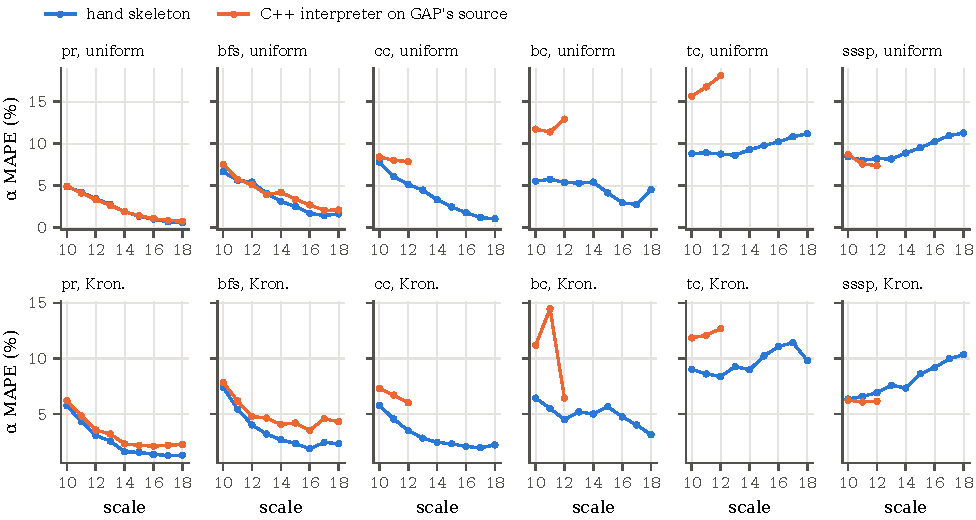
\includegraphics[width=\linewidth]{figures/gap_auto_vs_hand.pdf}
\caption[C++ interpreter against the hand skeleton, per scale]{$\alpha$ MAPE per scale: hand skeleton against the C++
interpreter on GAP's source, six kernels, uniform (top) and Kronecker (bottom) graphs.}
\label{fig:gap-auto}
\end{figure}

\begin{figure}[!htbp]
\centering
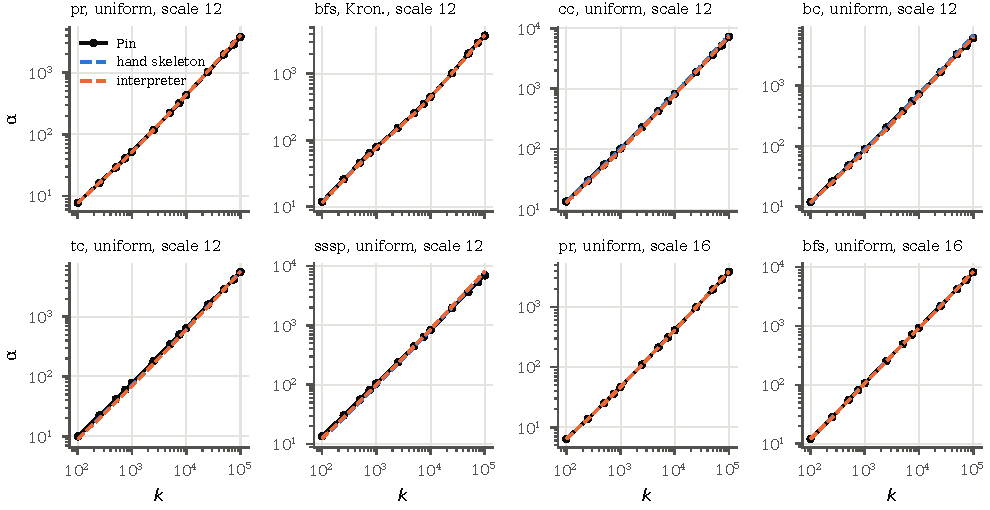
\includegraphics[width=\linewidth]{figures/gap_alpha_curves.pdf}
\caption[Predicted and measured $\alpha$ curves on GAP]{$\alpha$ against the interval: Pin, the hand skeleton and the
interpreter, for eight workload--scale pairs.}
\label{fig:gap-alpha}
\end{figure}

\begin{figure}[!htbp]
\centering
\begin{minipage}[t]{0.49\linewidth}
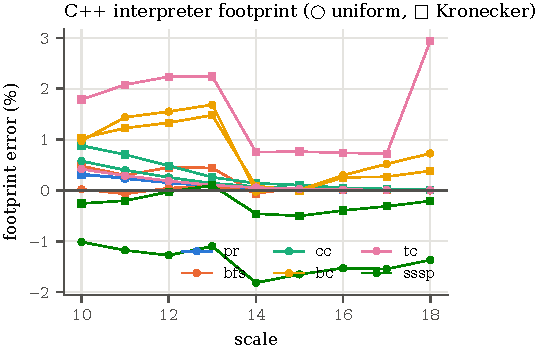
\includegraphics[width=\linewidth]{figures/gap_auto_footprint.pdf}
\caption[C++ interpreter footprint error]{Footprint error of the C++ interpreter per scale.}
\label{fig:gap-auto-fp}
\end{minipage}\hfill
\begin{minipage}[t]{0.49\linewidth}
\centering\scriptsize
\vspace{-12em}
\fittable{tables/auto_scales.tex}
\captionof{table}[pr and bfs per scale]{$\alpha$ MAPE (\%) per scale, pr and bfs.}
\label{tab:auto-scales}
\end{minipage}
\end{figure}

\begin{figure}[!htbp]
\centering
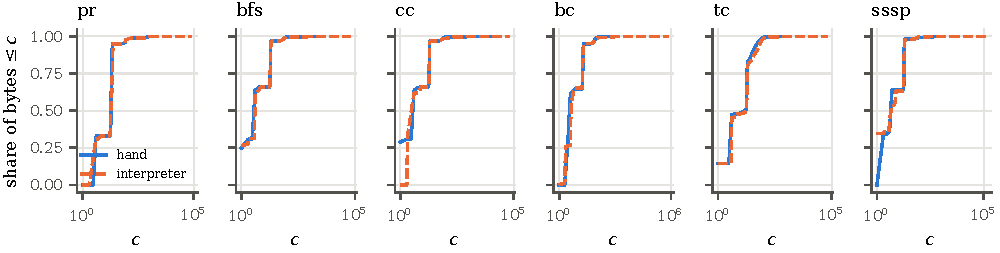
\includegraphics[width=\linewidth]{figures/gap_spectra.pdf}
\caption[Hand and interpreter spectra]{Cumulative spectra at scale 12 (uniform): hand skeleton against the
interpreter.}
\label{fig:gap-spectra}
\vspace{0.8em}
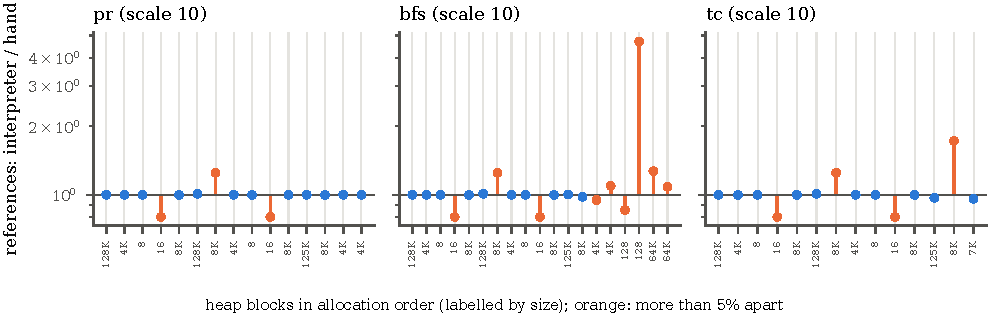
\includegraphics[width=\linewidth]{figures/gap_arrays.pdf}
\caption[Per-block comparison]{References to each heap block, interpreter over hand skeleton, at scale 10.}
\label{fig:gap-arrays}
\end{figure}

\subsection{Cost}

The first version of the interpreter took about 13 minutes at scale 16 and 67--78 minutes at scale 18, almost all
of it in GAP's prefix sum, which ran one vertex at a time. With scans, cached libclang answers (child lists, kinds
and canonical types are cached on the cursor and type objects, declaration keys on the declaration) and counting
over the touched range only, pr and bfs take about 20\,s at scale 16 and 1--2 minutes at scale 18; all 108
(kernel, graph, scale) runs took 39 minutes with 6 in parallel (\figref{fig:interp-cost}, \tabref{tab:cost}),
peaking at 12~GB in total. tc remains the slowest (18 minutes at scale 18 on Kronecker graphs): its merge loops
break per point and run one iteration at a time.

\begin{figure}[!htbp]
\centering
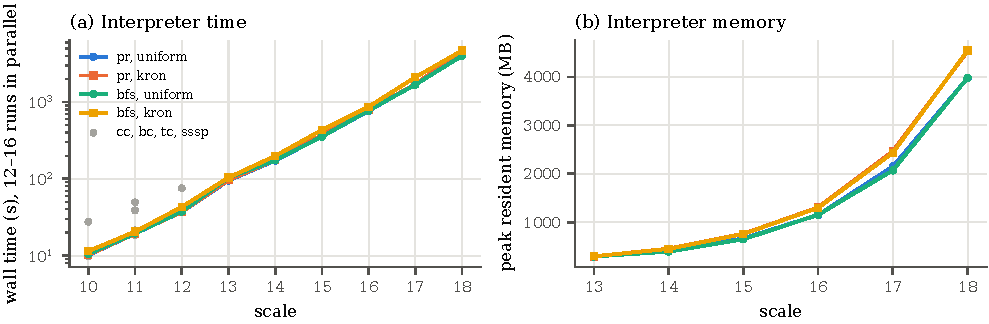
\includegraphics[width=\linewidth]{figures/interp_cost.pdf}
\caption[Cost of the C++ interpreter]{Wall time of the C++ interpreter per kernel, graph and scale.}
\label{fig:interp-cost}
\end{figure}

\begin{table}[!htbp]
\centering\small
\caption{C++ interpreter seconds per kernel and scale (u: uniform, K: Kronecker; 6 runs in parallel).}
\label{tab:cost}
\fittable{tables/cost.tex}
\end{table}

%=====================================================================
\clearpage
\section{A blind test on programs never seen in development}
\label{sec:blind}

Everything so far was developed against the workloads it was scored on, or (GAP's large scales) against the same
programs. To test whether the interpreter generalises to code it was not built for, we chose two programs that
generate their input from their command line and were never used in development, ran them in the interpreter
without any trace of them, committed the predictions, and only then traced them
(\code{paper\_generalization/blind/PROTOCOL.md}):
\begin{itemize}
\item \textbf{HPCCG} (Mantevo, \code{80dd2f1}): conjugate gradient on a 27-point stencil matrix generated for an
$n^3$ grid; 150 CG iterations (tolerance 0); serial, \code{-O3}; $n = 10, 12, 14, 16, 20, 24, 28$.
\item \textbf{LULESH 2.0} (LLNL, \code{3e01c40}): Lagrangian shock hydrodynamics on an $s^3$ hexahedral mesh, 11
material regions with load-imbalance repetitions, 20 cycles; serial, \code{-O3}; $s = 5, 8, 10, 12, 15, 18, 20$.
\end{itemize}

\paragraph{Protocol.} Bringing the two programs up in the interpreter, before any trace, exposed generic gaps
(floating-point values in memory, scans of pointers, command-line strings, unity builds, default construction of
\code{std::vector} members, and four defects); they were fixed and the interpreter frozen at commit
\code{20a8d1e}. The runtime baseline was fitted on the 12 serial GAP workloads (same compiler, libstdc++ and glibc),
the heap started from GAP's measured state, and the predictions were committed at \code{2757a35}. Only then were the
programs traced and scored; the predictions were not changed. The interpreter takes 11--48\,s per HPCCG input and
39\,s--5 minutes per LULESH input; coverage is 1.0 for HPCCG and 0.954 for LULESH.

\begin{table}[!htbp]
\centering\small
\caption[Blind test per config]{Blind test: predicted against traced footprint and $\alpha$ MAPE per config. The last
column is LULESH after the post-hoc fix (partial values).}
\label{tab:blind}
\fittable{tables/blind.tex}
\end{table}

\begin{table}[!htbp]
\centering\small
\caption[Blind test against the own model]{Blind test against each program's own MemPrint model (trained on its other
six configs), $\alpha$ MAPE (\%) at the held-out config.}
\label{tab:blind-splits}
\fittable{tables/blind_splits.tex}
\end{table}

\begin{figure}[!htbp]
\centering
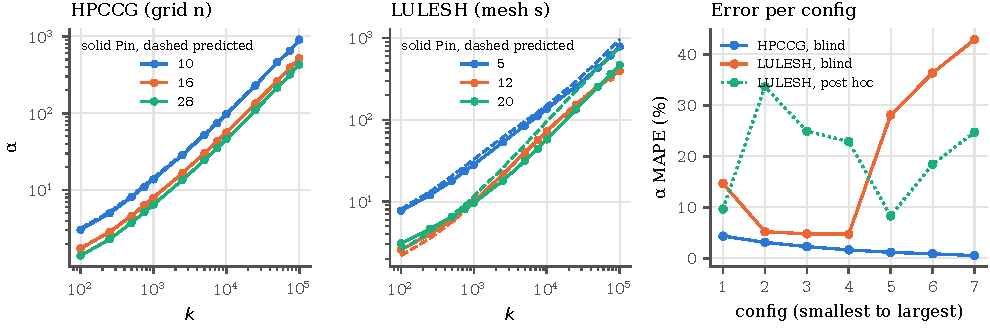
\includegraphics[width=\linewidth]{figures/blind.pdf}
\caption[Blind test]{Blind test. Left and middle: $\alpha$ against the interval, traced (solid) and predicted before
tracing (dashed), for three configs of each program. Right: $\alpha$ MAPE per config.}
\label{fig:blind}
\end{figure}

\paragraph{Results.} (\tabref{tab:blind}, \tabref{tab:blind-splits}, \figref{fig:blind}.)
\begin{itemize}
\item \textbf{HPCCG passes clearly.} The footprint is within $+0.09$ to $+2.1\%$ and $\alpha$ within 0.5--4.4\% at
every grid size, improving with size as the runtime baseline becomes a smaller share. With the largest grid held out,
the prediction from source is 0.53\% off against 12.2\% for the program's own model trained on its six other traced
sizes; with the middle grid held out, 1.66\% against 11.1\%.
\item \textbf{LULESH passes partly.} The footprint is within $-4.2$ to $-0.4\%$ at every mesh size, and $\alpha$
within 4.7--5.2\% at $s = 8, 10, 12$ (INTER: 4.74\% against the own model's 17.0\%). At $s = 15, 18, 20$, however,
$\alpha$ is 28--43\% off (EXTRA: 42.9\% against 7.9\%): the predicted spectrum has too few heavily referenced bytes
(at $k = 10^5$, $\alpha$ is 758 predicted and 467 measured at $s = 20$).
\end{itemize}

\paragraph{Post hoc.} Looking for the cause after the traces existed, we found that a variable assigned in the
branches of an \code{if}/\code{else} taken by different regions (LULESH's \code{rep}, how many times a region's
equation of state is evaluated: 1, 2 or 20) stayed unknown, so those loops were charged one trip. Partial values fix
this (GAP is unchanged by it), and LULESH's error at $s = 15$--$20$ falls to 8--25\%, but at $s = 8$--$12$ it rises to
23--34\% (\tabref{tab:blind}, last column). The good middle sizes of the blind run therefore benefited from errors that
cancelled, and LULESH's remaining error has more than one cause; the strongest candidate is that local coordinate
arrays filled by a nested loop do not keep per-iteration values across the nested batch, so some floating-point
time-step and cut-off decisions stay unknown (coverage 0.95--0.98). We report the blind numbers as the result.

%=====================================================================
\clearpage
\section{Discussion}
\label{sec:discussion}

\paragraph{How code translates into $z$.}
The chain is: code $\to$ (abstract execution) $\to$ spectrum $\to$ (\eqref{eq:moments}) $\to$ bin moments $\to$
$z$. Only the first arrow needs the program; the rest is arithmetic. Which static features matter is therefore not a
modelling choice: they are whatever determines how many references each byte receives. For affine code this is the
loop bounds and subscripts; for generated irregular inputs, the generator's distribution and the kernel's control
flow on it. Syntactic summaries (AST node counts) predict transfer poorly because they do not determine the spectrum.

\paragraph{Predict rather than borrow.}
Once the spectrum is available, borrowing a model is unnecessary: the static $\alpha$ beats every borrowed model,
including the oracle. Similarity in $\zhat$ remains useful where the static prediction is not trusted but some
program's model must be chosen, and as an out-of-distribution signal (miniVite).

\paragraph{What generalises.}
Generic and reusable: the moment formulas, the per-unit counting, the glibc model, the library cost curves (sort,
Mersenne Twister, \code{rand}), the interpreters' batch execution, the \code{-O3} register and load model and the
container models. Specific to a program: only the stub table of command-line values. The hand skeletons were specific
to GAP; the C++ interpreter replaces them.

\paragraph{Threats to validity.}
\begin{itemize}
\item The uniform-graph pr and bfs skeleton results were tuned on their own traces; the Kronecker, new-kernel and
thread tests were blind. The interpreter results on GAP were compared with Pin while the interpreter was being
developed (scales 10--12 for all kernels); its pr and bfs results at scales 13--18 were not used during development.
HPCCG and LULESH (\secref{sec:blind}) are the only fully blind test of the interpreter, and two programs are a small
sample.
\item The \code{rand()} cost and the floyd-warshall/nussinov sequential execution were added after their errors were
seen.
\item One runtime per suite: the baseline is shared because the programs share a compiler, C library and harness. A
program with a different runtime needs its own baseline or the gate.
\item The splitter's subsamples come from one execution per input; run-to-run variation of the program is not in
the bins.
\end{itemize}

\paragraph{Limitations.}
\begin{itemize}
\item No symbolic counting. Counting with Polly~\cite{grosser2012polly} and Barvinok~\cite{verdoolaege2007barvinok}
would make affine spectra independent of input size; the interpreter enumerates instead, in time proportional to the
references charged.
\item Inputs read from files are outside the approach; only inputs generated from a known distribution are.
\item Floating-point values are tracked in scalars and memory but not across every batching path (a nested batch that
fills a local array), and values computed differently from the compiled code (vectorised sums, fused multiply-add) can
take a different branch near a tie. Converging PageRank (prc) is left out of the interpreter route.
\item Code that the interpreter does not model (other library containers, I/O-driven control, MPI) falls to the gate.
\end{itemize}

%=====================================================================
\section{Related work}
\label{sec:related}

\paragraph{Sampling memory references.}
Trace sampling for cache simulation~\cite{kessler1994} and statistical cache models~\cite{Berg2013StatCache,
eklov2010statstack} estimate miss ratios from sampled reuse; SHARDS~\cite{waldspurger2015shards} samples by hashed
address to build miss-ratio curves. Phase-based sampling~\cite{sherwood2002simpoint,wunderlich2003smarts} reduces
simulation cost by selecting representative intervals. \memprint{}~\cite{memprint} samples references for the
footprint and learns the correction per program; this report removes the per-program training.

\paragraph{Locality from program structure.}
Reuse-distance analysis~\cite{mattson1970,Beyls2005ReuseDistance,ding2003reuse} characterises locality, and
Ding and Zhong predict whole-program locality across inputs from a few training runs. The working set
model~\cite{denning1968} relates footprint to time windows. Polyhedral tools count the integer points of iteration
domains and access relations symbolically~\cite{grosser2012polly,verdoolaege2007barvinok}, which yields exact
access counts for affine code; our interpreter computes the same quantity by enumeration and extends it to irregular
code with generated inputs.

\paragraph{Instrumentation.}
Pin~\cite{Luk2005Pin}, Valgrind~\cite{Nethercote2007Valgrind} and its heap profilers~\cite{ValgrindMassif,dhat}
measure memory exactly at high cost; MemGaze~\cite{Xu2020MemGaze} samples traces with hardware support.

%=====================================================================
\section{Conclusion}
\label{sec:conclusion}

For a program that has never been traced, the footprint and \memprint{}'s correction factor $\alpha$ can be
predicted from its source code: under Bernoulli sampling both follow in closed form from the access-count spectrum,
and the spectrum can be computed by executing the source abstractly, with a small shared baseline for the runtime.
On PolyBench this beats every alternative that borrows another program's model and even the program's own model.
The same spectrum yields a descriptor of memory behaviour whose distances rank model transfer as well as measured
behaviour does. For irregular programs with generated inputs, replaying the program on input drawn from the
generator's distribution works, first with hand-written skeletons and now with a C++ interpreter that runs the
benchmark's own source.

\paragraph{Reproducibility.}
Everything in this report is regenerated by
\begin{lstlisting}
python paper_generalization/compute.py                                # data/*.csv
python paper_generalization/make_figures.py                           # figures/*.pdf
python paper_generalization/make_tables.py                            # tables/*.tex
\end{lstlisting}
from the traces and spectra in \code{data/} (commands for producing those are in the repository's
\code{FINDINGS.md}).

\clearpage
\bibliographystyle{plain}
\bibliography{references}

\appendix
\section{Per-kernel leave-one-out results}

\begin{table}[!htbp]
\centering\scriptsize
\caption[Per-kernel leave-one-out results]{Per held-out PolyBench kernel: footprint error (fp), static $\alpha$ and own
model MAPE (\%) for both splits, and, for EXTRA, the known kernel nearest by $\zhat$ and the oracle.}
\label{tab:lowo-kernel}
\fittable{tables/lowo_per_kernel.tex}
\end{table}

\section{Commands}
\begin{lstlisting}
# PolyBench, traced with bytes touched
scripts/run.sh polybench --mode splitter --footprint bytes --runs 1 --bench <kernel>
python -m memprint --root data/polybench-bytes preprocess
python -m memprint --root data/polybench-bytes static spectra --polybench workloads/src/polybench
python -m memprint --root data/polybench-bytes static idioms --polybench workloads/src/polybench
python -m memprint --root data/polybench-bytes static lowo --ast <ast_features.csv> --transfer miniVite
# GAP
scripts/run.sh gapbs --mode splitter --footprint bytes --runs 1 --configs "10 11 12 13 14 15 16 17 18"
python -m memprint --root data/gap-bytes preprocess
python -m memprint --root data/gap-bytes static gap --borrow data/polybench-bytes/data
# C programs
python -m memprint --root data/csr-bytes static programs --borrow data/polybench-bytes/data
\end{lstlisting}

\end{document}
